\newpage\section{Diagrammi dei casi d'uso}

\subsection{UC1: Login e registrazione}
\begin{center}
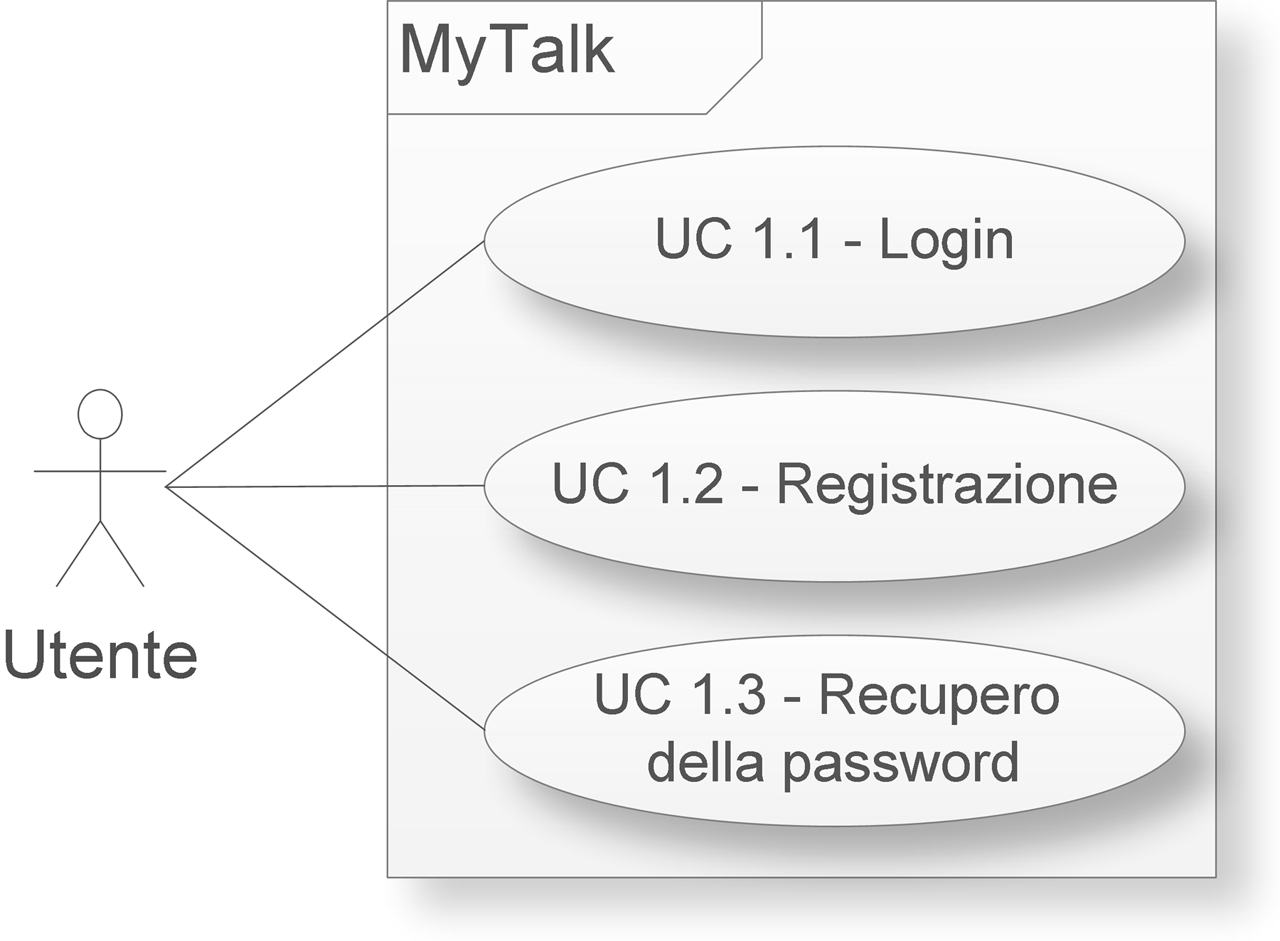
\includegraphics[width=.5\textwidth]{UC1}
\end{center}
\begin{description}
\item{\scshape\bfseries Attori principali:}Utente.
\item{\scshape\bfseries Scopo e descrizione:} L'utente può effettuare l'accesso al sistema mediante la procedura di login se registrato, recuperare la password dimenticata oppure può provvedere alla propria registrazione, quindi effettuare successivamente l'accesso al sistema.
\item{\scshape\bfseries Precondizione:} Il sistema MyTalk è attivo e funzionante, le infrastrutture di rete sono attive.
\item{\scshape\bfseries Postcondizione:} Una volta eseguita la procedura di login (previa eventuale registrazione o recupero password) un utente generico diviene un utente autenticato.
\item{\scshape\bfseries Illustrazione scenario principale:} Se in possesso delle credenziali, l'utente le inserisce nella schermata di login e conferma la propria volontà di effettuare l'accesso al sistema. Nel caso in cui non dovesse essere in possesso delle credenziali perché le ha smarrite, viene avviata la procedura di recupero password. Se invece la mancata disponibilità delle credenziali è dovuta al fatto che l'utente non si è mai registrato al sistema, viene avviata la procedura di registrazione.
\item{\scshape\bfseries Illustrazione scenario alternativo:} Durante la registrazione o login il sistema può fallire. Il sistema evidenzia gli errori riscontrati e l'utente rimane nella pagina fino alla risoluzione degli errori. Può inoltre succedere che le infrastrutture di rete non risultano più attive: viene visualizzato un messaggio d'errore che notifica l'impossibilità di effettuare l'operazione richiesta.
\end{description}

\subsection{UC1.1: Login utente}
\begin{center}
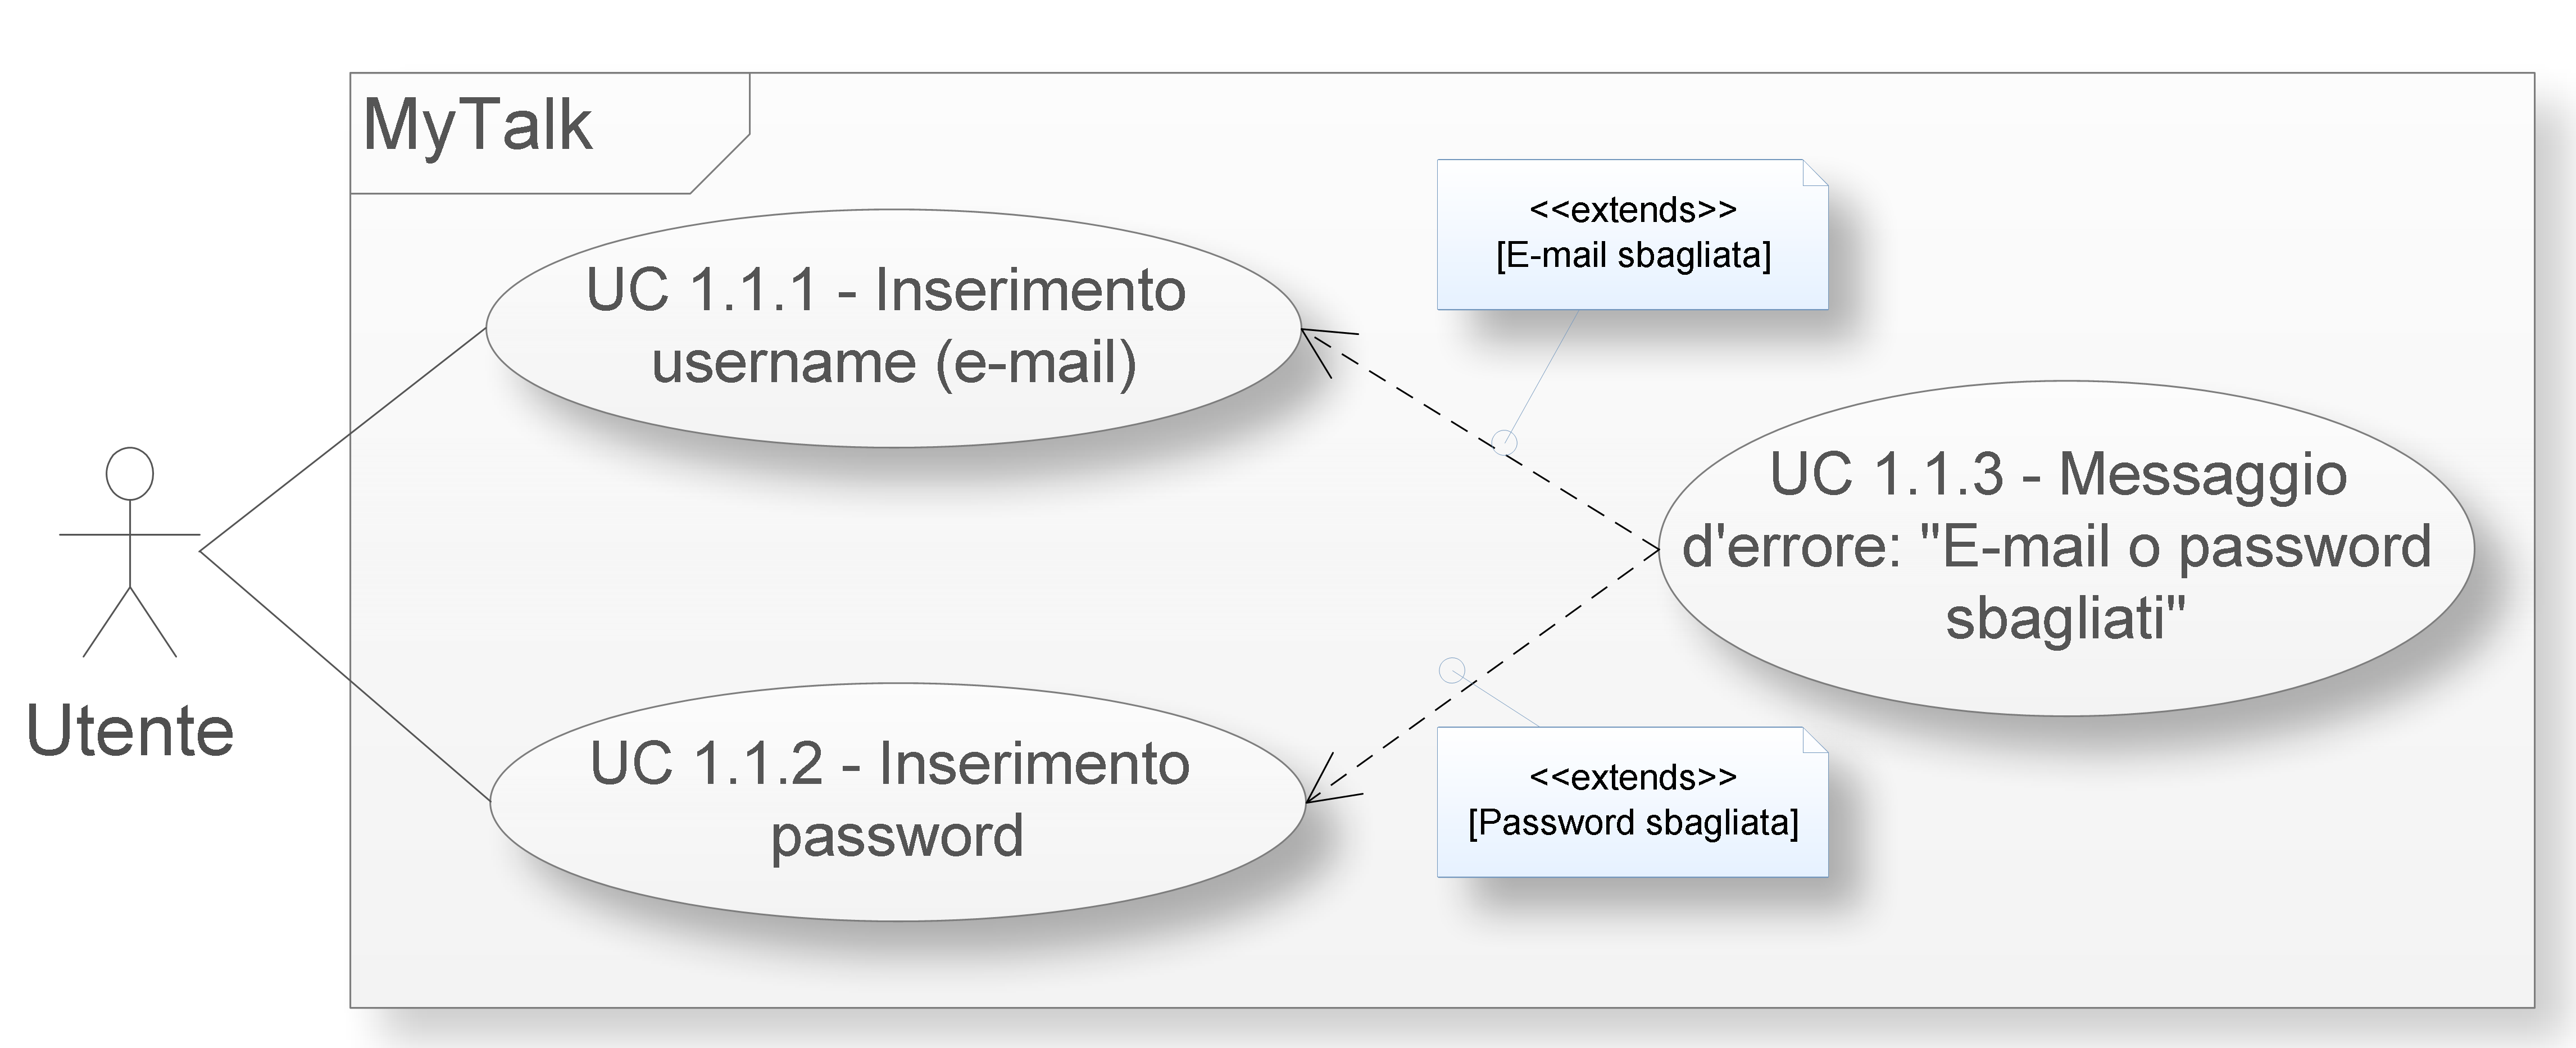
\includegraphics[width=.9\textwidth]{UC1-1}
\end{center}
\begin{description}
\item{\scshape\bfseries Attori principali:}Utente.
\item{\scshape\bfseries Scopo e descrizione:} L'utente si autentica per accedere al sistema MyTalk
\item{\scshape\bfseries Precondizione:} L'utente (generico) visualizza la schermata iniziale e il sistema è pronto.
\item{\scshape\bfseries Postcondizione:} L'utente si è loggato nel sistema
\item{\scshape\bfseries Illustrazione scenario principale:} L'utente si trova nella pagina principale e deve inserire le credenziali d'accesso (e-mail e password) per poter utilizzare le funzionalità.
\item{\scshape\bfseries Illustrazione scenario alternativo:} L'utente ha inserito dati non corretti: il sistema lo notifica con un errore e rimane in attesa di una correzione.
\end{description}

\subsection{UC1.2: Registrazione}
\begin{center}
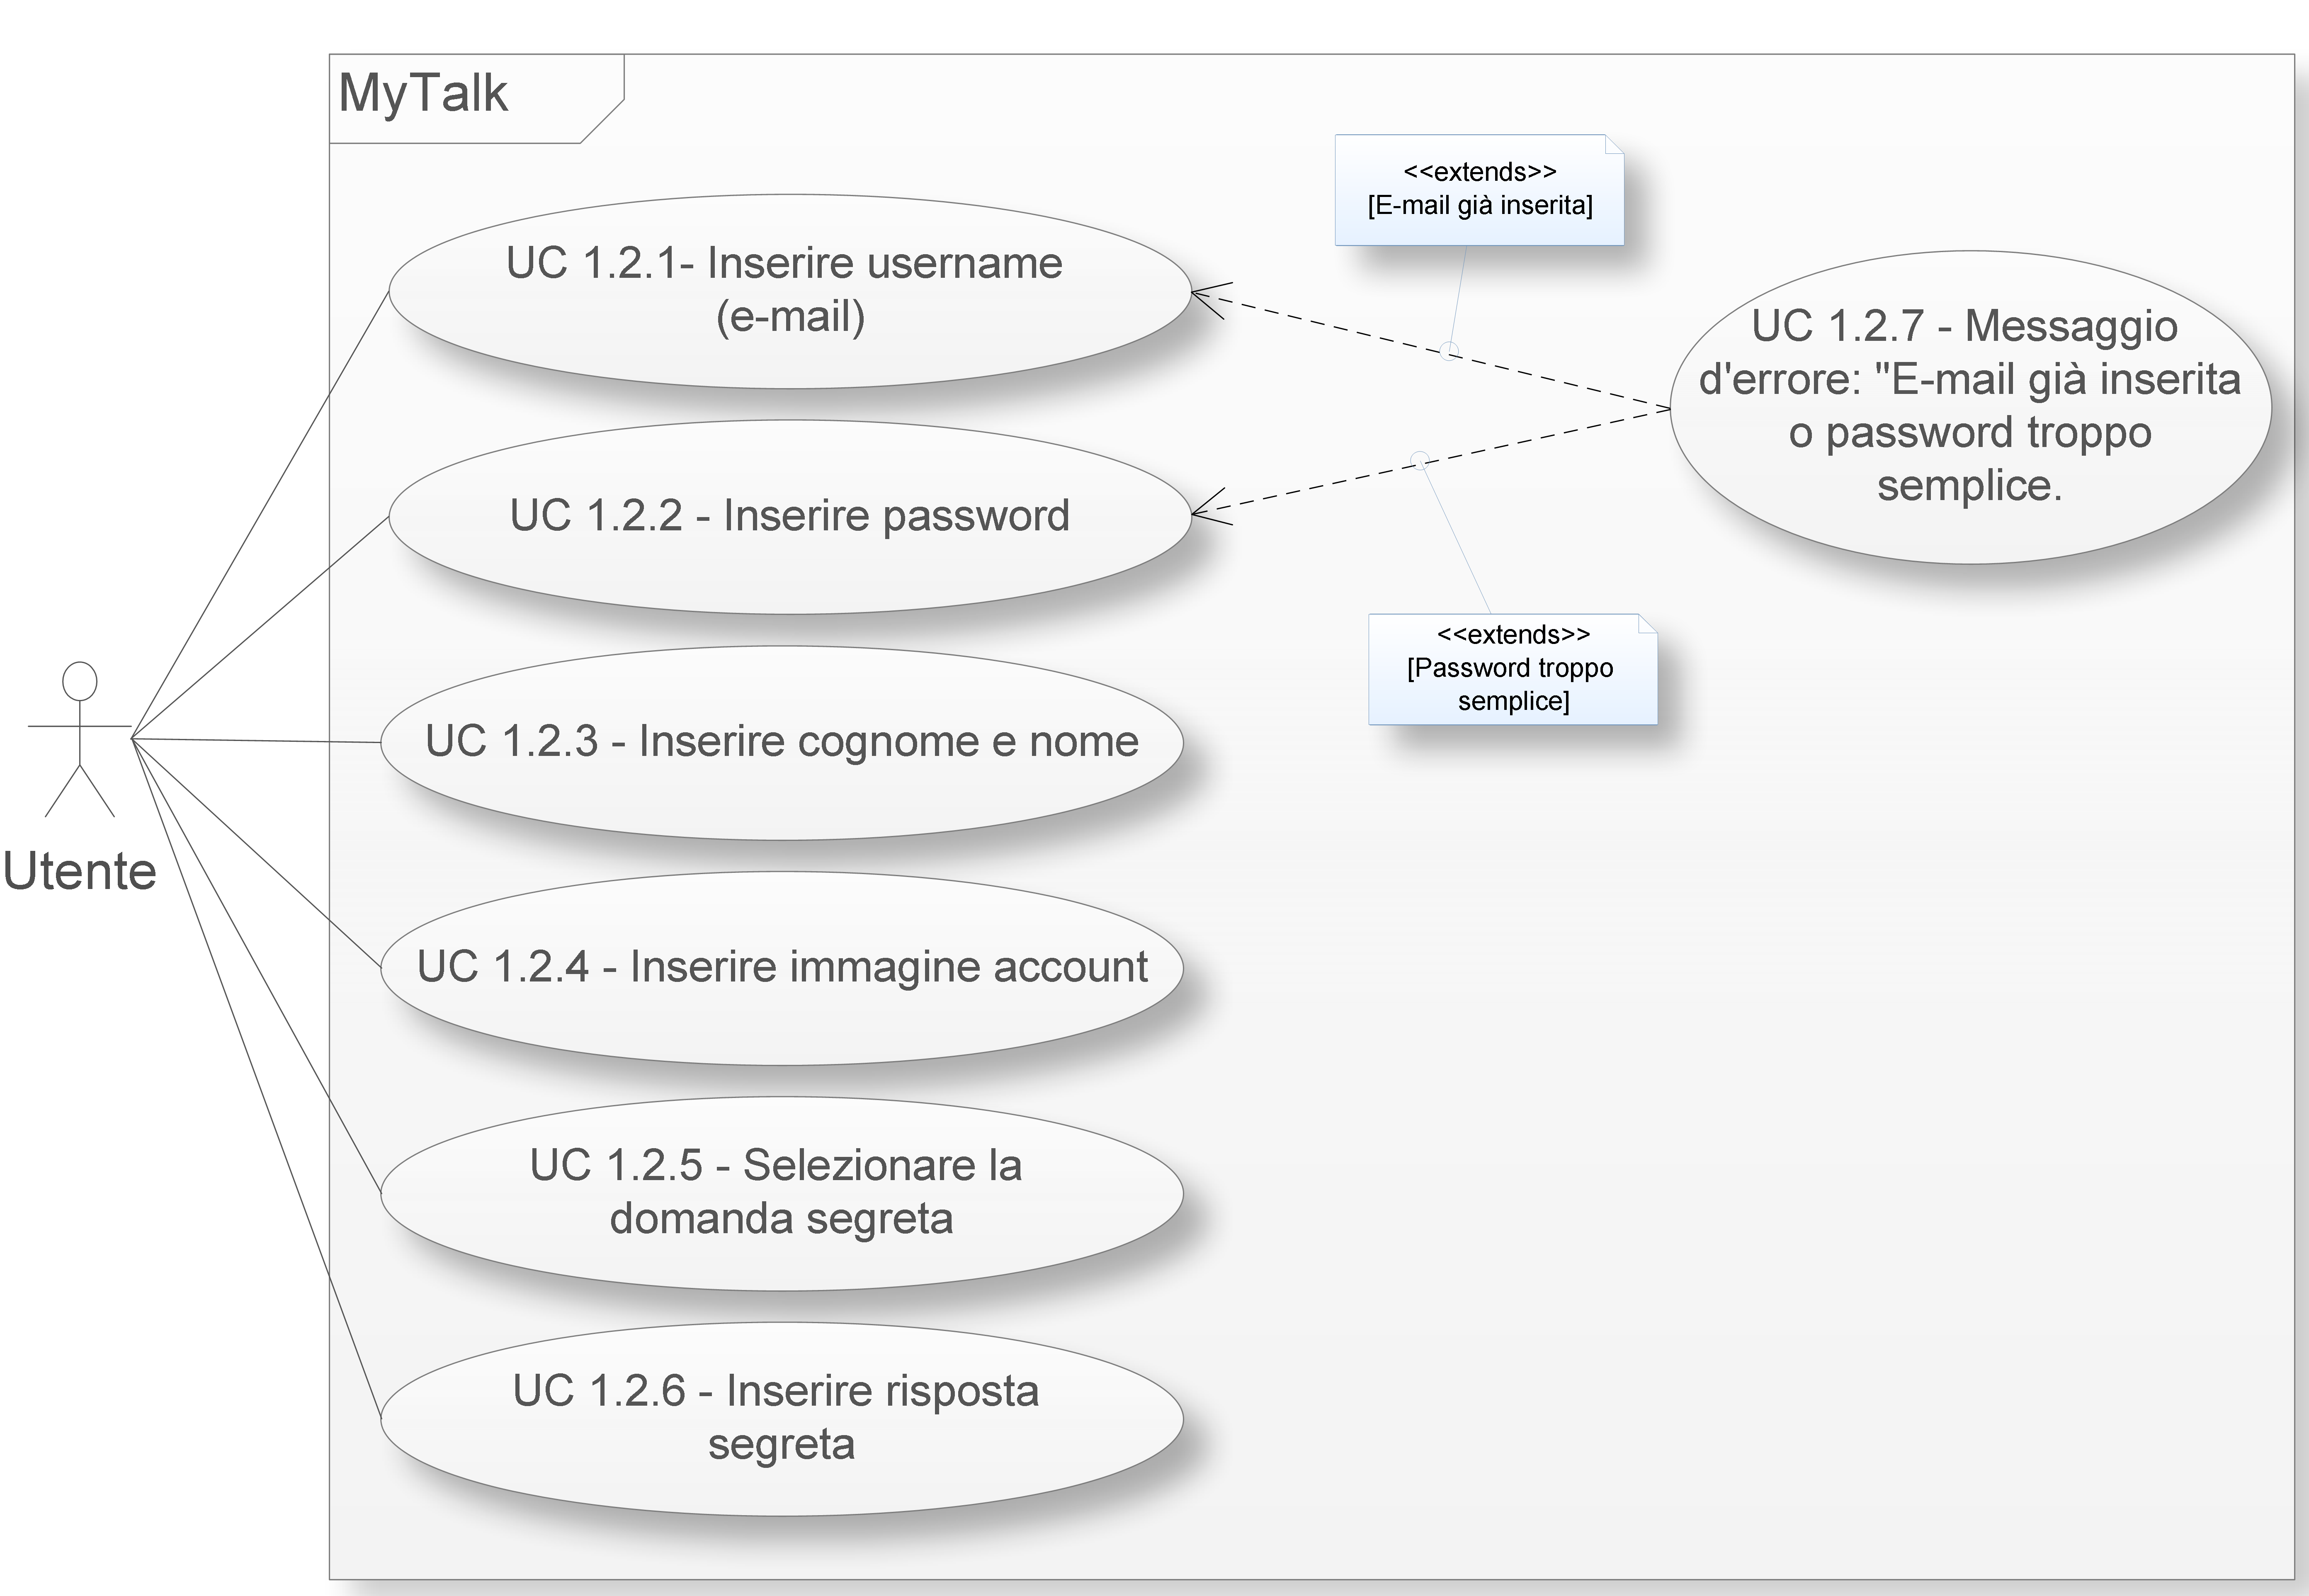
\includegraphics[width=.9\textwidth]{UC1-2}
\end{center}
\begin{description}
\item{\scshape\bfseries Attori principali:}Utente.
\item{\scshape\bfseries Scopo e descrizione:} L'utente si registra nel sistema.
\item{\scshape\bfseries Precondizione:} L'utente (generico) visualizza la schermata iniziale e il sistema è pronto.
\item{\scshape\bfseries Postcondizione:} L'utente si è registrato nel sistema MyTalk
\item{\scshape\bfseries Illustrazione scenario principale:} La registrazione di un nuovo account comporta l'inserimento di un indirizzo email come ID utente, una password, e un'immagine da associare al proprio profilo. Per andare a buon fine la procedura di registrazione richiede che la password prescelta assicuri un sufficiente livello di complessità e prevede altresì la selezione della domanda segreta (e della relativa risposta) necessarie al recupero della password in caso di smarrimento, nonché la validazione dell'indirizzo email al fine di verificare che l'utente ne sia effettivamente in possesso.
\item{\scshape\bfseries Illustrazione scenario alternativo:} Il sistema può fallire per via dell'inserimento di dati non corretti. Il sistema evidenzia gli errori e rimane in attesa della correzione.
\end{description}

\subsection{UC1.3: Recupero della password}
\begin{center}
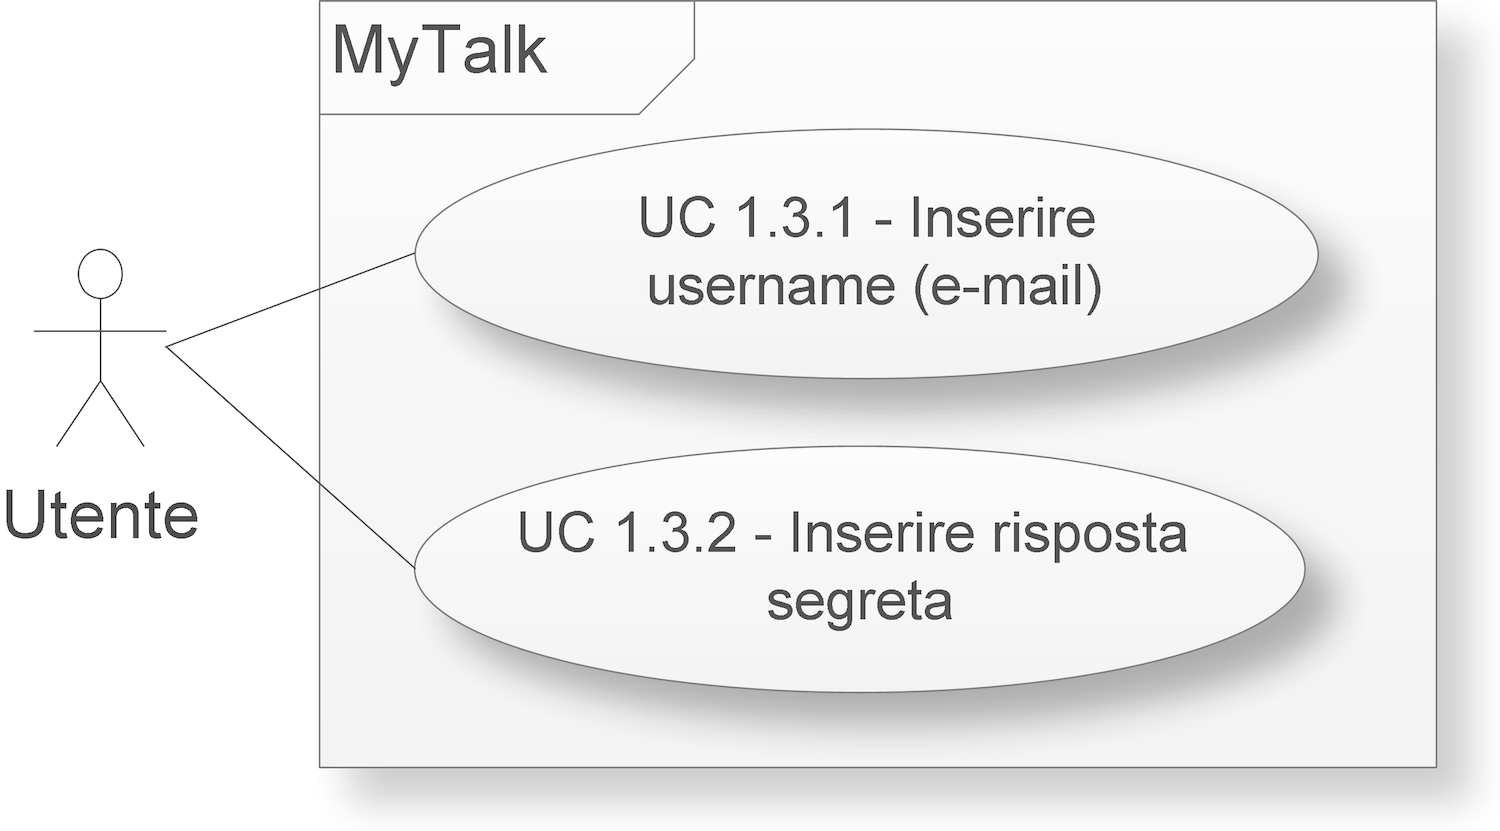
\includegraphics[width=.5\textwidth]{UC1-3}
\end{center}
\begin{description}
\item{\scshape\bfseries Attori principali:}Utente.
\item{\scshape\bfseries Scopo e descrizione:} L'utente desidera recuperare la password smarrita.
\item{\scshape\bfseries Precondizione:} L'utente (generico) visualizza la schermata iniziale e il sistema è pronto.
\item{\scshape\bfseries Postcondizione:} L'utente riceve per e-mail la password dimenticata.
\item{\scshape\bfseries Illustrazione scenario principale:} Si avvia la procedura di recupero della password: l'utente deve inserire l'e-mail e la risposta alla domanda segreta. A questo segue l'invio della password all'indirizzo email indicato in fase di registrazione.
\item{\scshape\bfseries Illustrazione scenario alternativo:} Il sistema può fallire per via dell'inserimento di dati non corretti. Il sistema evidenzia gli errori e rimane in attesa della correzione.
\end{description}

\subsection{UC2: Home screen dell'applicativo}
\begin{center}
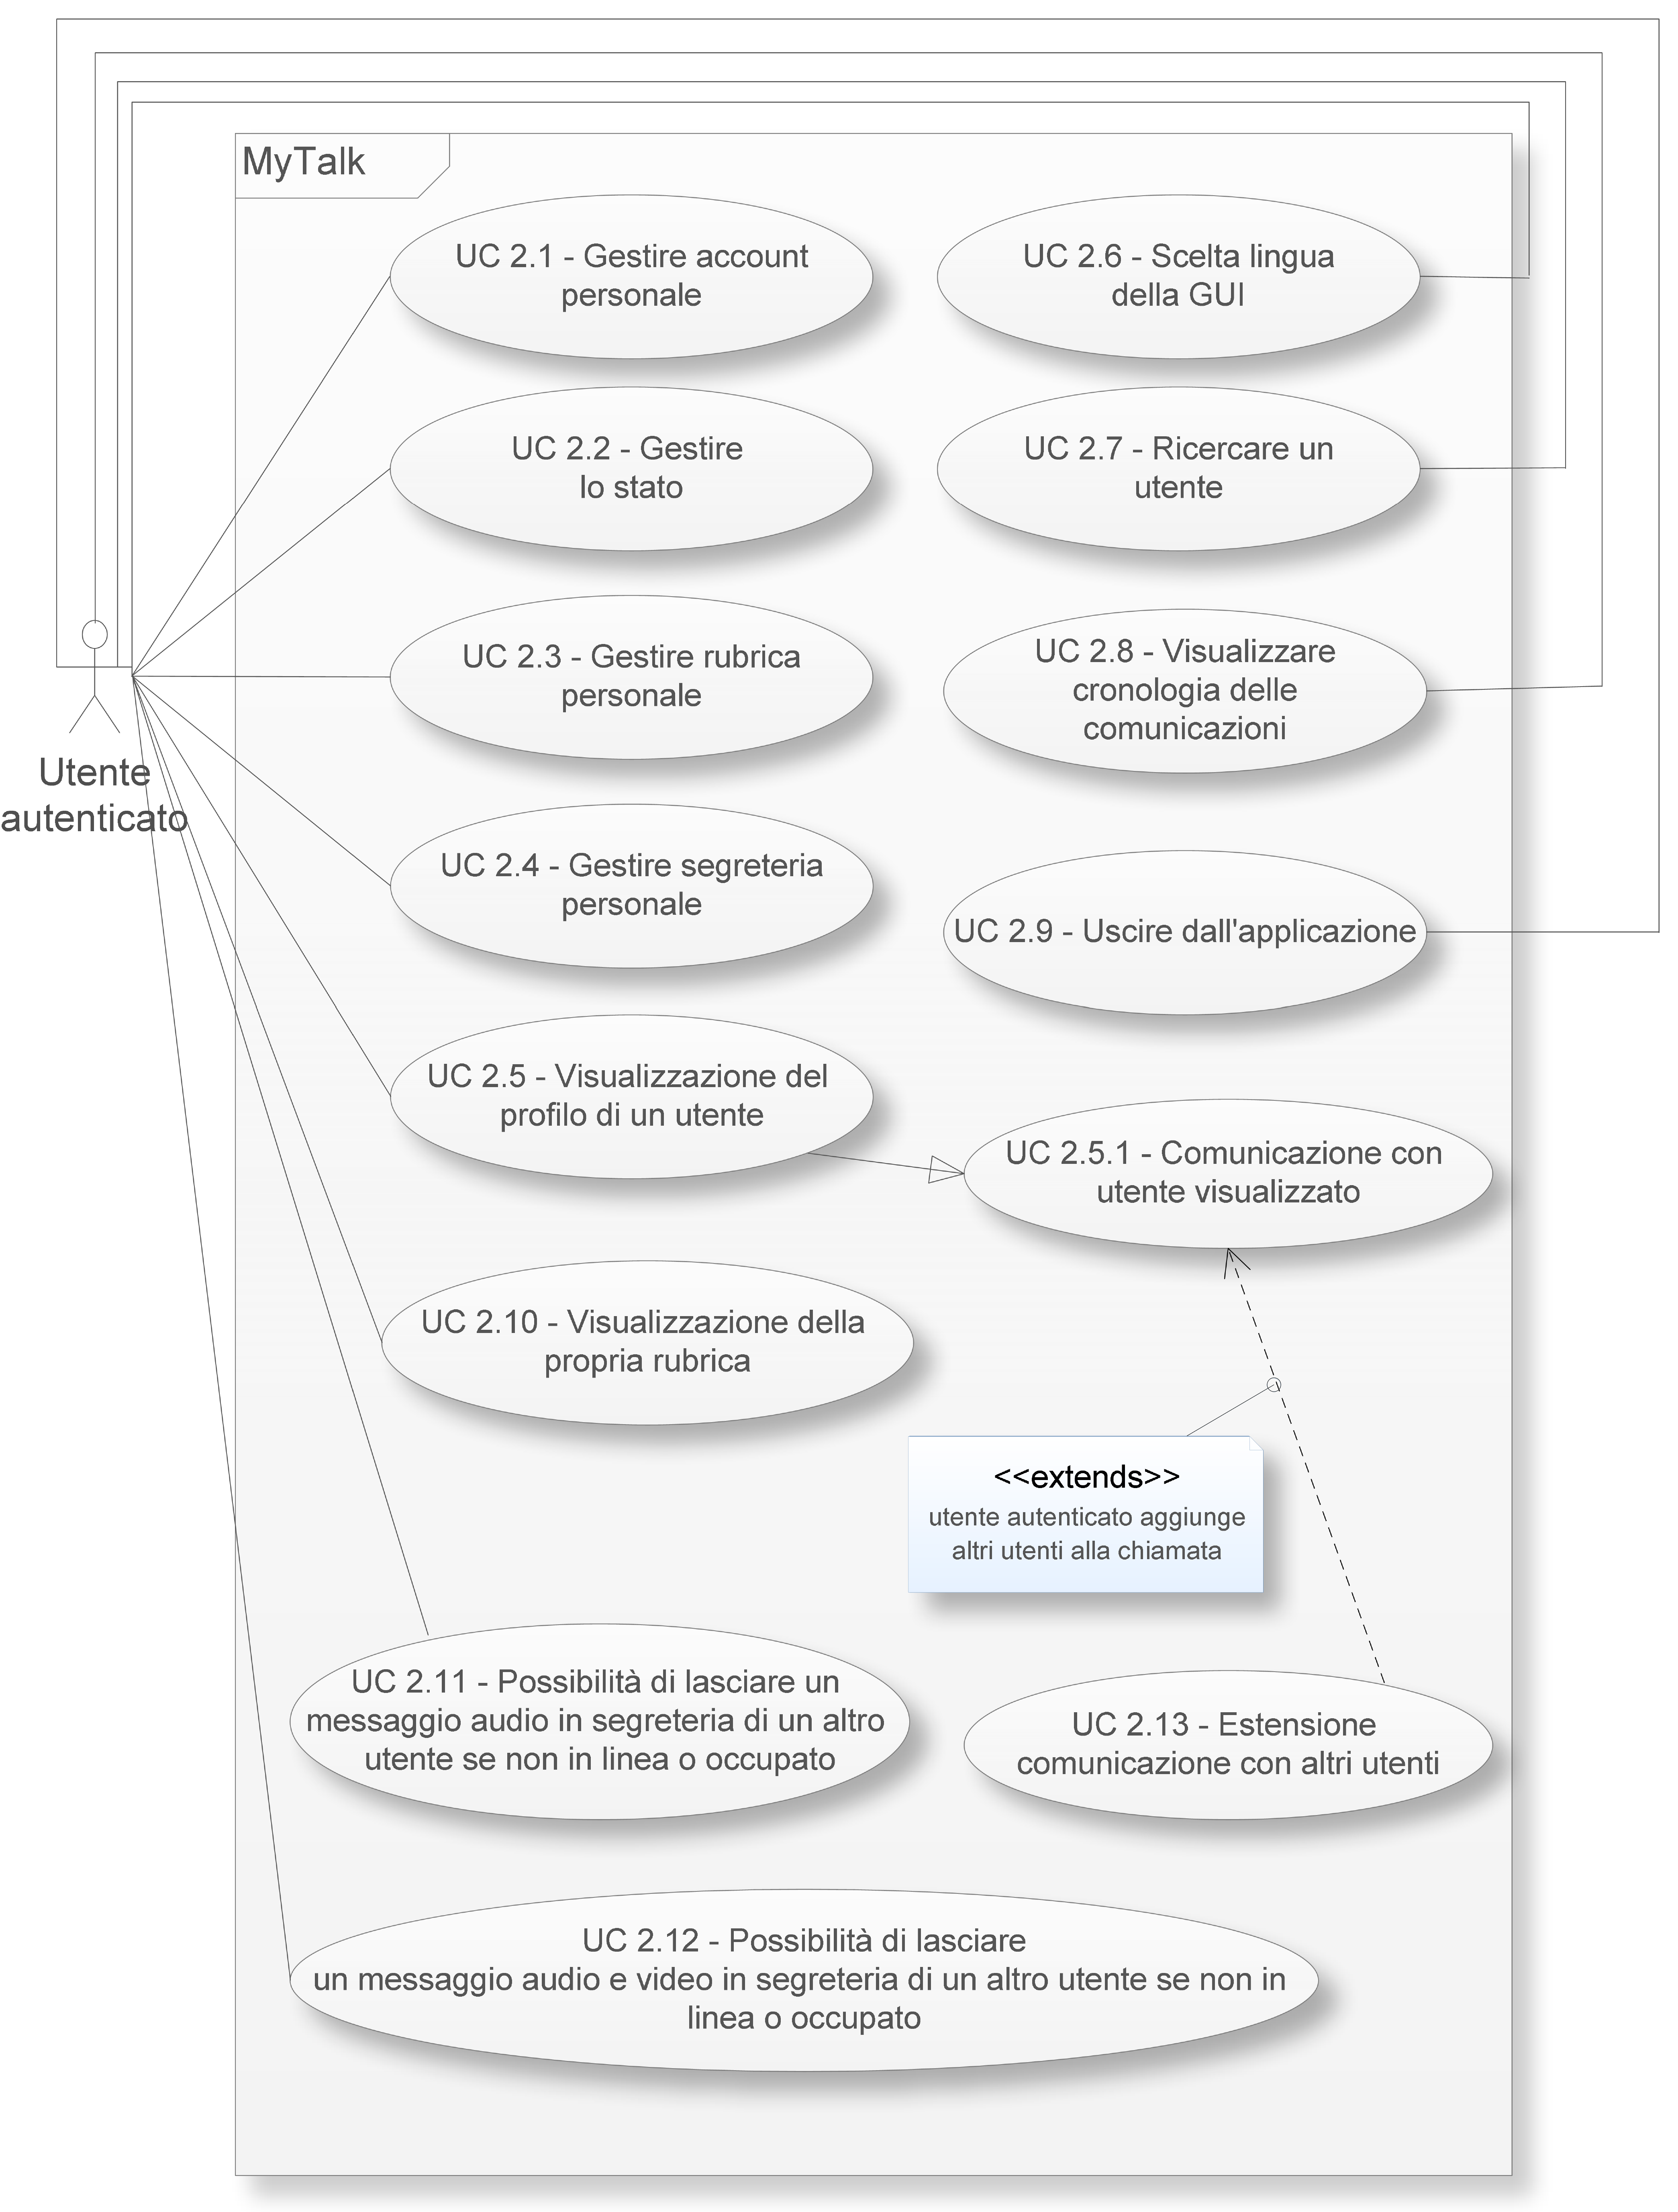
\includegraphics[width=\textwidth]{UC2}
\end{center}
\begin{description}
\item{\scshape\bfseries Attori principali:}Utente autenticato.
\item{\scshape\bfseries Scopo e descrizione:} Funzionalità generali offerte all'utente autenticato e presenti nella Home screen dell'applicativo.
\item{\scshape\bfseries Precondizione:} L'utente ha eseguito il login ed è autenticato nel sistema.
\item{\scshape\bfseries Postcondizione:} L'utente ha eseguito una delle funzioni proposte.
\item{\scshape\bfseries Illustrazione scenario principale:} L'utente dopo aver eseguito il login al sistema, si trova nella Home dell'applicativo. Qui può svolgere una delle seguenti opzioni: gestire il proprio account, scegliere la lingua della GUI, gestire lo stato, eseguire delle ricerche di utenti, gestire la propria rubrica, lasciare un messaggio nella segreteria di un utente, gestire la propria segreteria, visualizzare la cronologia delle comunicazioni, stabilire connessioni con altri utenti che si specializza in una connessione audio, audio/video o chat, visualizzare gli utenti registrati nel sistema e, se è già stata aperta una connessione, può estenderla ad altri utenti. Infine l'utente ha la possibilità di chiudere l'applicativo.
\end{description}

\subsection{UC2.1: Gestione account}
\begin{center}
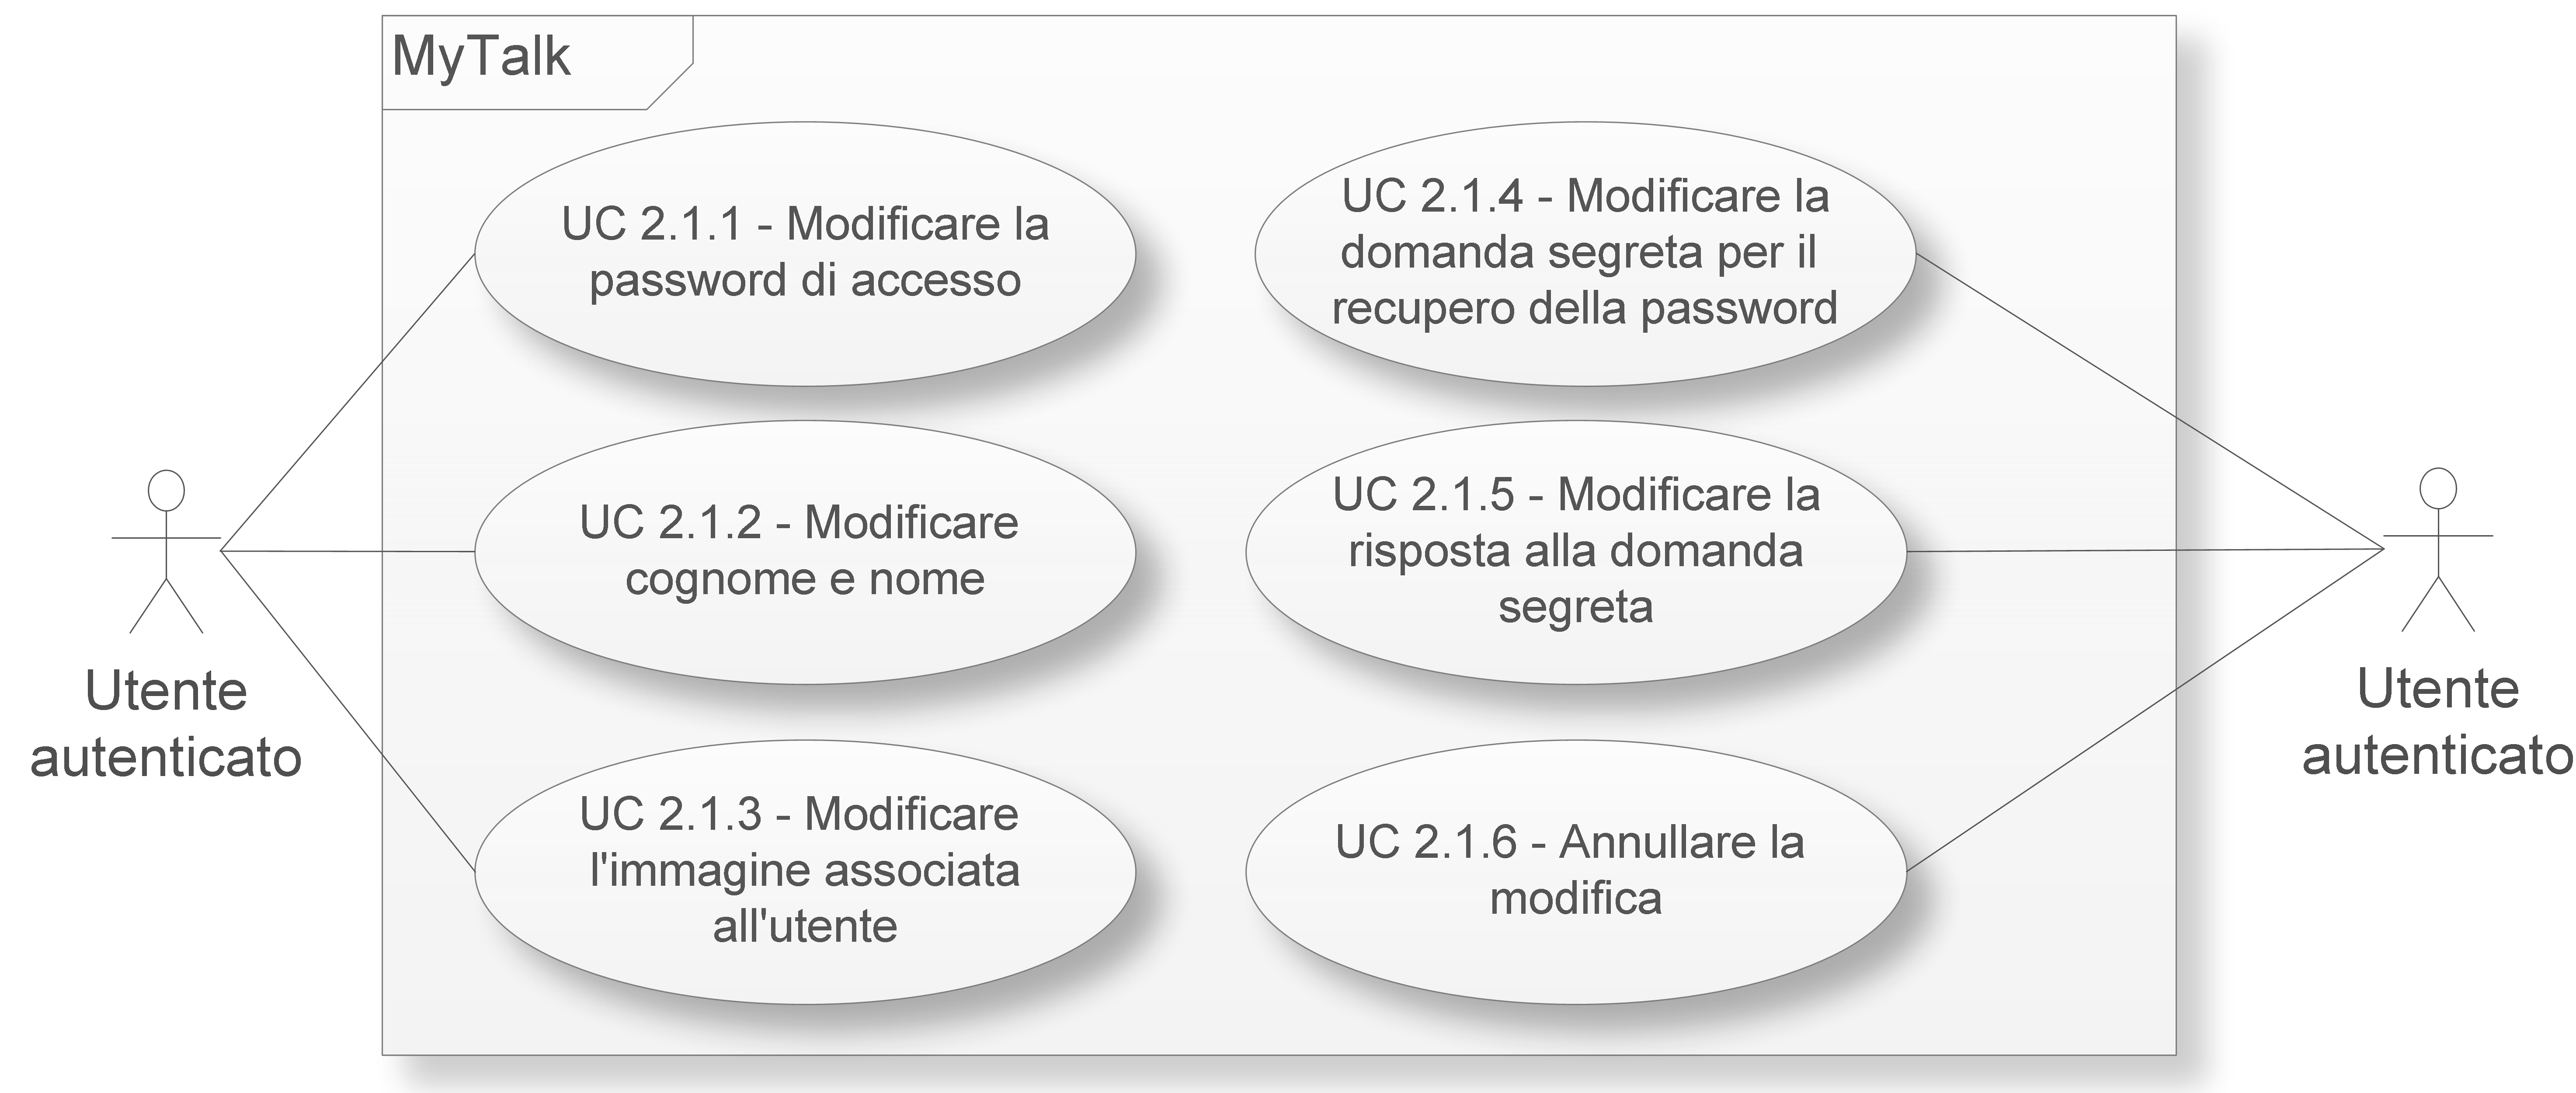
\includegraphics[width=.9\textwidth]{UC2-1}
\end{center}
\begin{description}
\item{\scshape\bfseries Attori principali:}Utente autenticato.
\item{\scshape\bfseries Scopo e descrizione:} un utente autenticato, ha la possibilità di modificare i propri dati personali, inseriti durante la sua registrazione, così da rimediare ad eventuali errori.
\item{\scshape\bfseries Precondizione:} l'utente corrente e' registrato nel sistema, ed ha effettuato il login.
\item{\scshape\bfseries Postcondizione:} i dati dell'utente sono stati aggiornati con i valori da lui inseriti.
\item{\scshape\bfseries Illustrazione scenario principale:} L'utente visualizza i valori correnti dei dati che lo riguardano e può apportare
le modifiche che ritiene necessarie. I dati che puo' modificare sono:
password;
nome;
cognome;
immagine profilo;
domanda segreta;
risposta alla domanda segreta;
Può quindi concludere salvando le modifiche.
\item{\scshape\bfseries Illustrazione scenario alternativo:} Prima del salvataggio l'utente può annullare l'operazione e, di conseguenza,
tornare alla schermata principale senza determinare alcun cambiamento al proprio
profilo.
\end{description}

\subsection{UC2.3: Gestione della rubrica}
\begin{center}
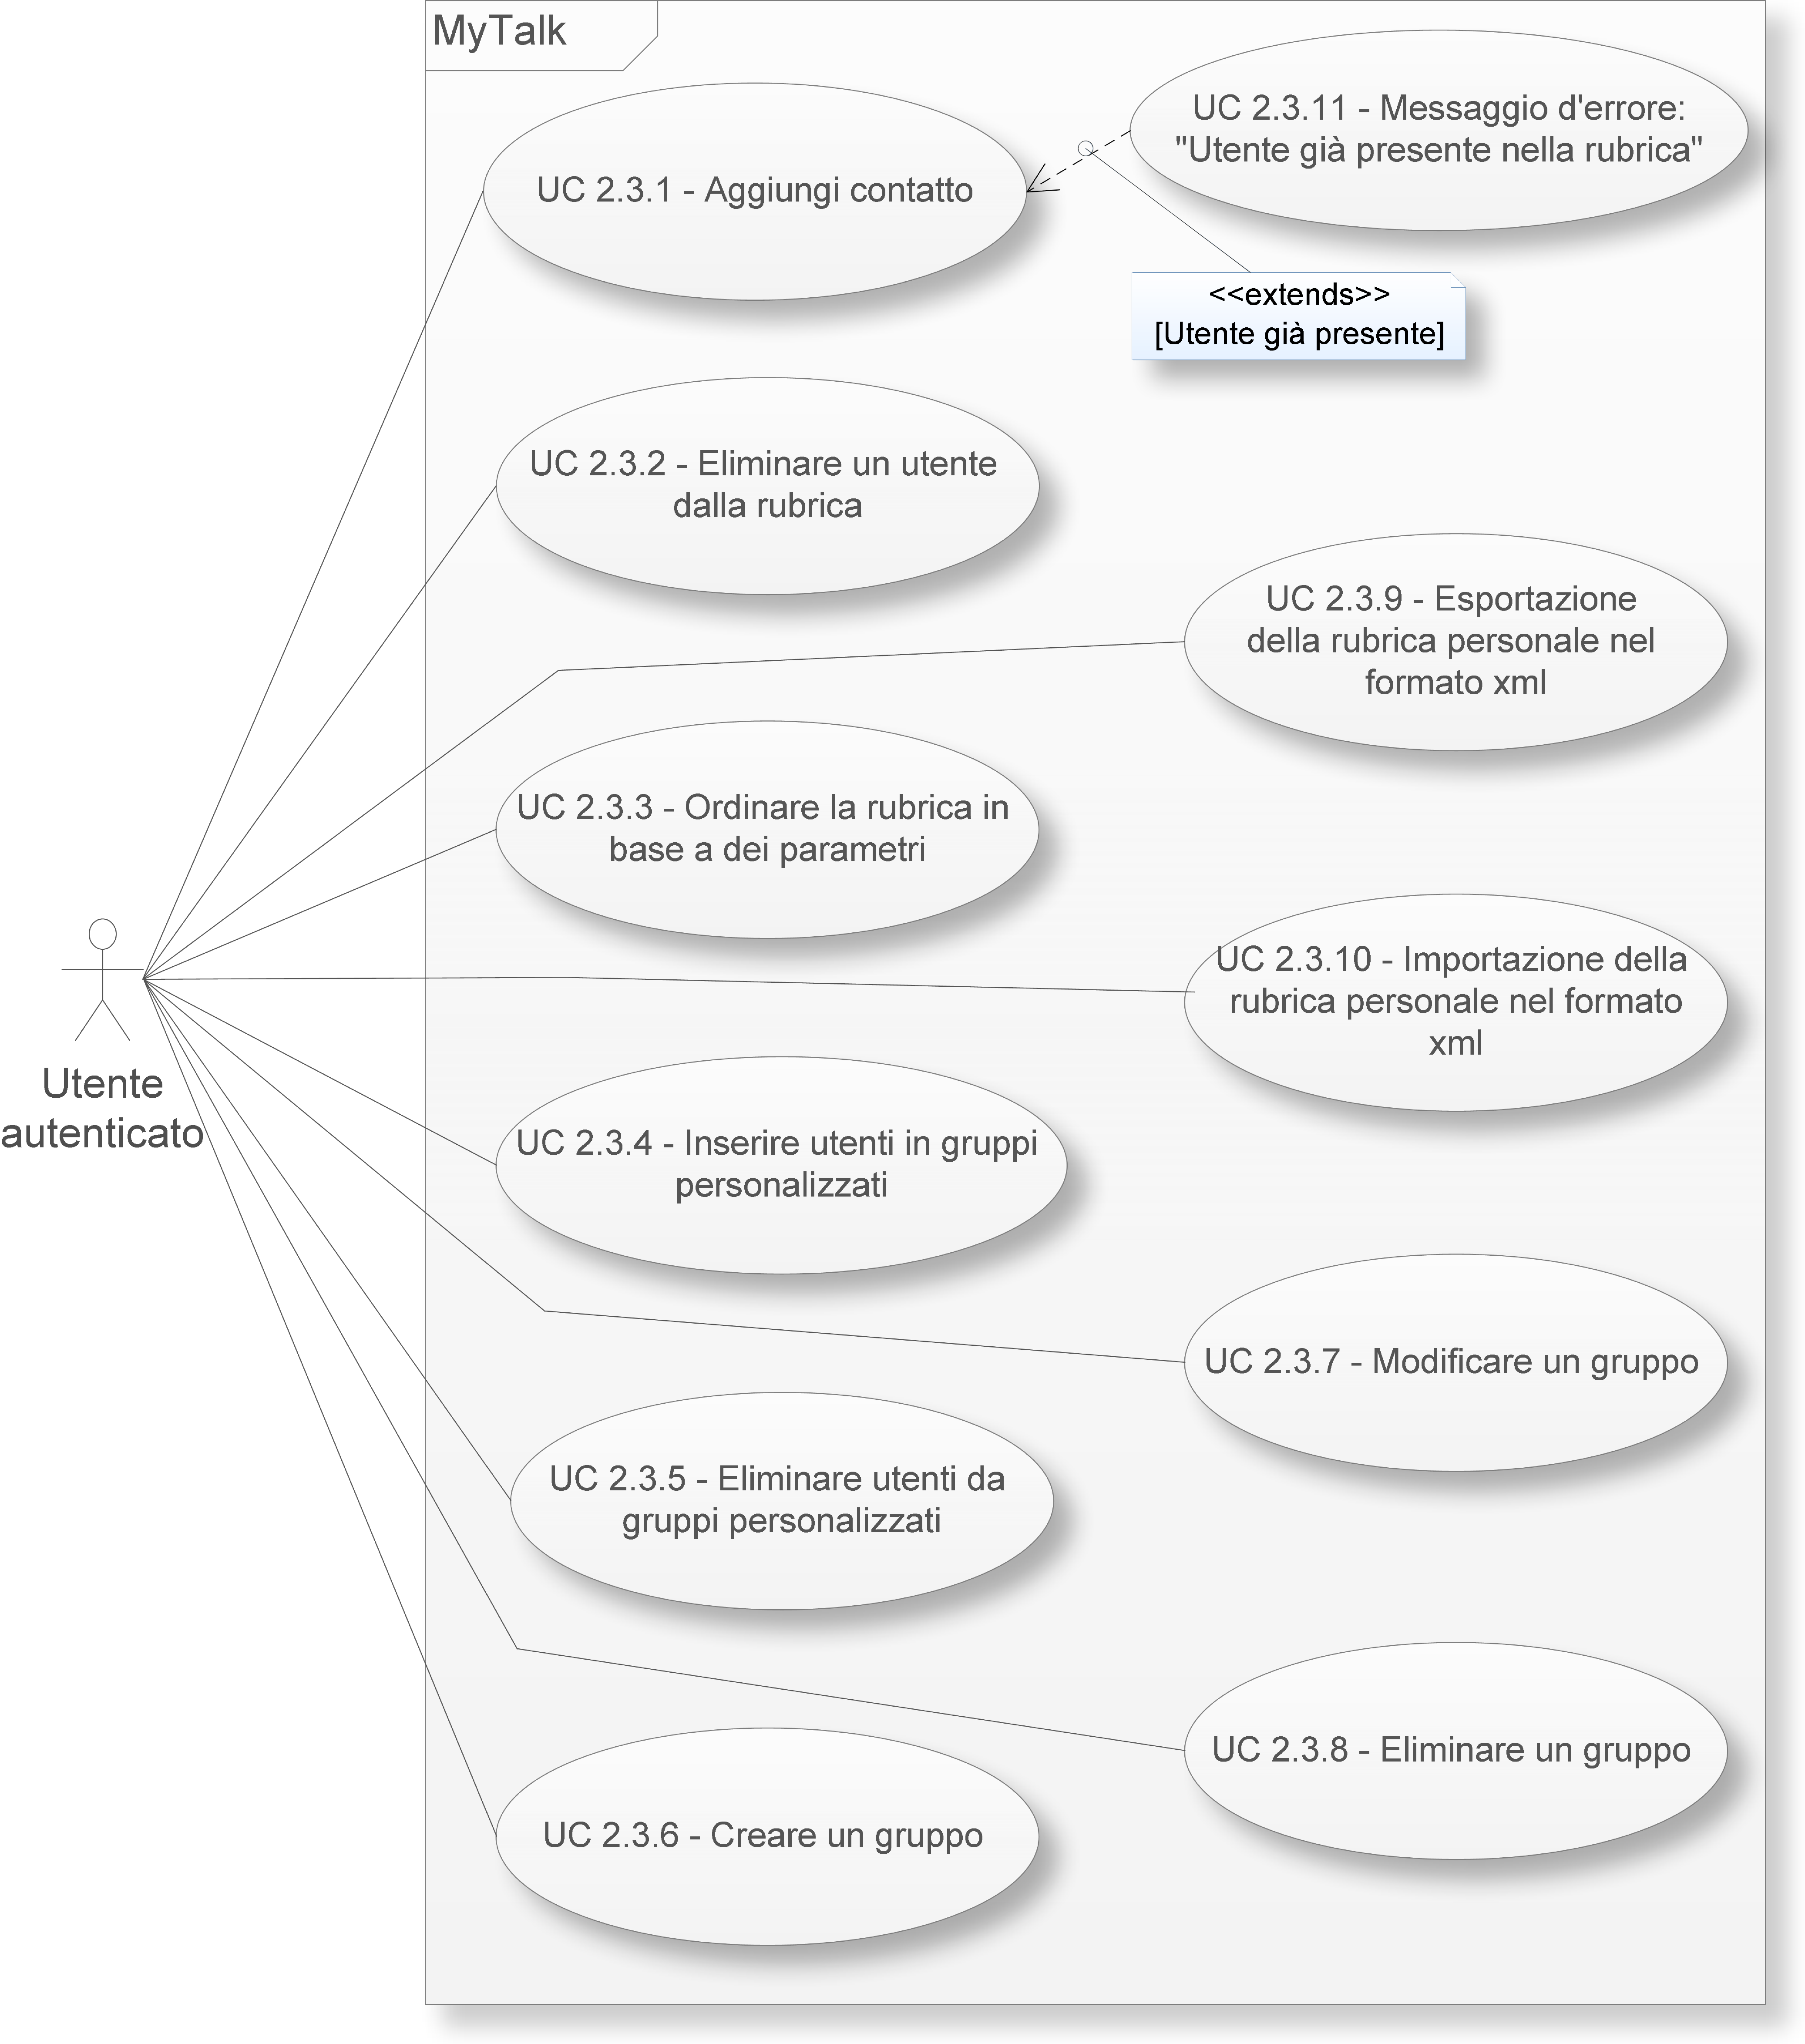
\includegraphics[width=.9\textwidth]{UC2-3}
\end{center}
\begin{description}
\item{\scshape\bfseries Attori principali:}Utente autenticato.
\item{\scshape\bfseries Scopo e descrizione:} L'utente può visualizzare ed organizzare la rubrica dei propri contatti personali sulla base della lista degli utenti che si sono registrati, oppure importando i contati da un file esterno.
\item{\scshape\bfseries Precondizione:} L'utente ha effettuato la procedura di login ed è quindi autenticato.
\item{\scshape\bfseries Postcondizione:} Se l'utente ha attuato delle modifiche, queste sono state salvate. Altrimenti non ci sono state modifiche sui dati inerenti la rubrica.
\item{\scshape\bfseries Illustrazione scenario principale:} L'utente visualizza la lista di utenti registrati al sistema, affiancata dalla propria rubrica divisa in gruppi. Quindi può scegliere una delle seguenti opzioni: aggiunge un contatto alla rubrica nel gruppo di default "contatti personali"; aggiunge un contatto alla rubrica nel gruppo di default "black-list"; crea un nuovo gruppo; elimina un gruppo; aggiunge un contatto alla rubrica in un gruppo scelto tra quelli già creati; elimina un contatto dalla propria rubrica;  sposta un utente presente in rubrica da un gruppo ad un altro; esporta i contatti presenti nella propria rubrica; importa dei contatti prelevati da un file .xml.
\end{description}

\subsection{UC2.3.1: Aggiungi contatto}
\begin{center}
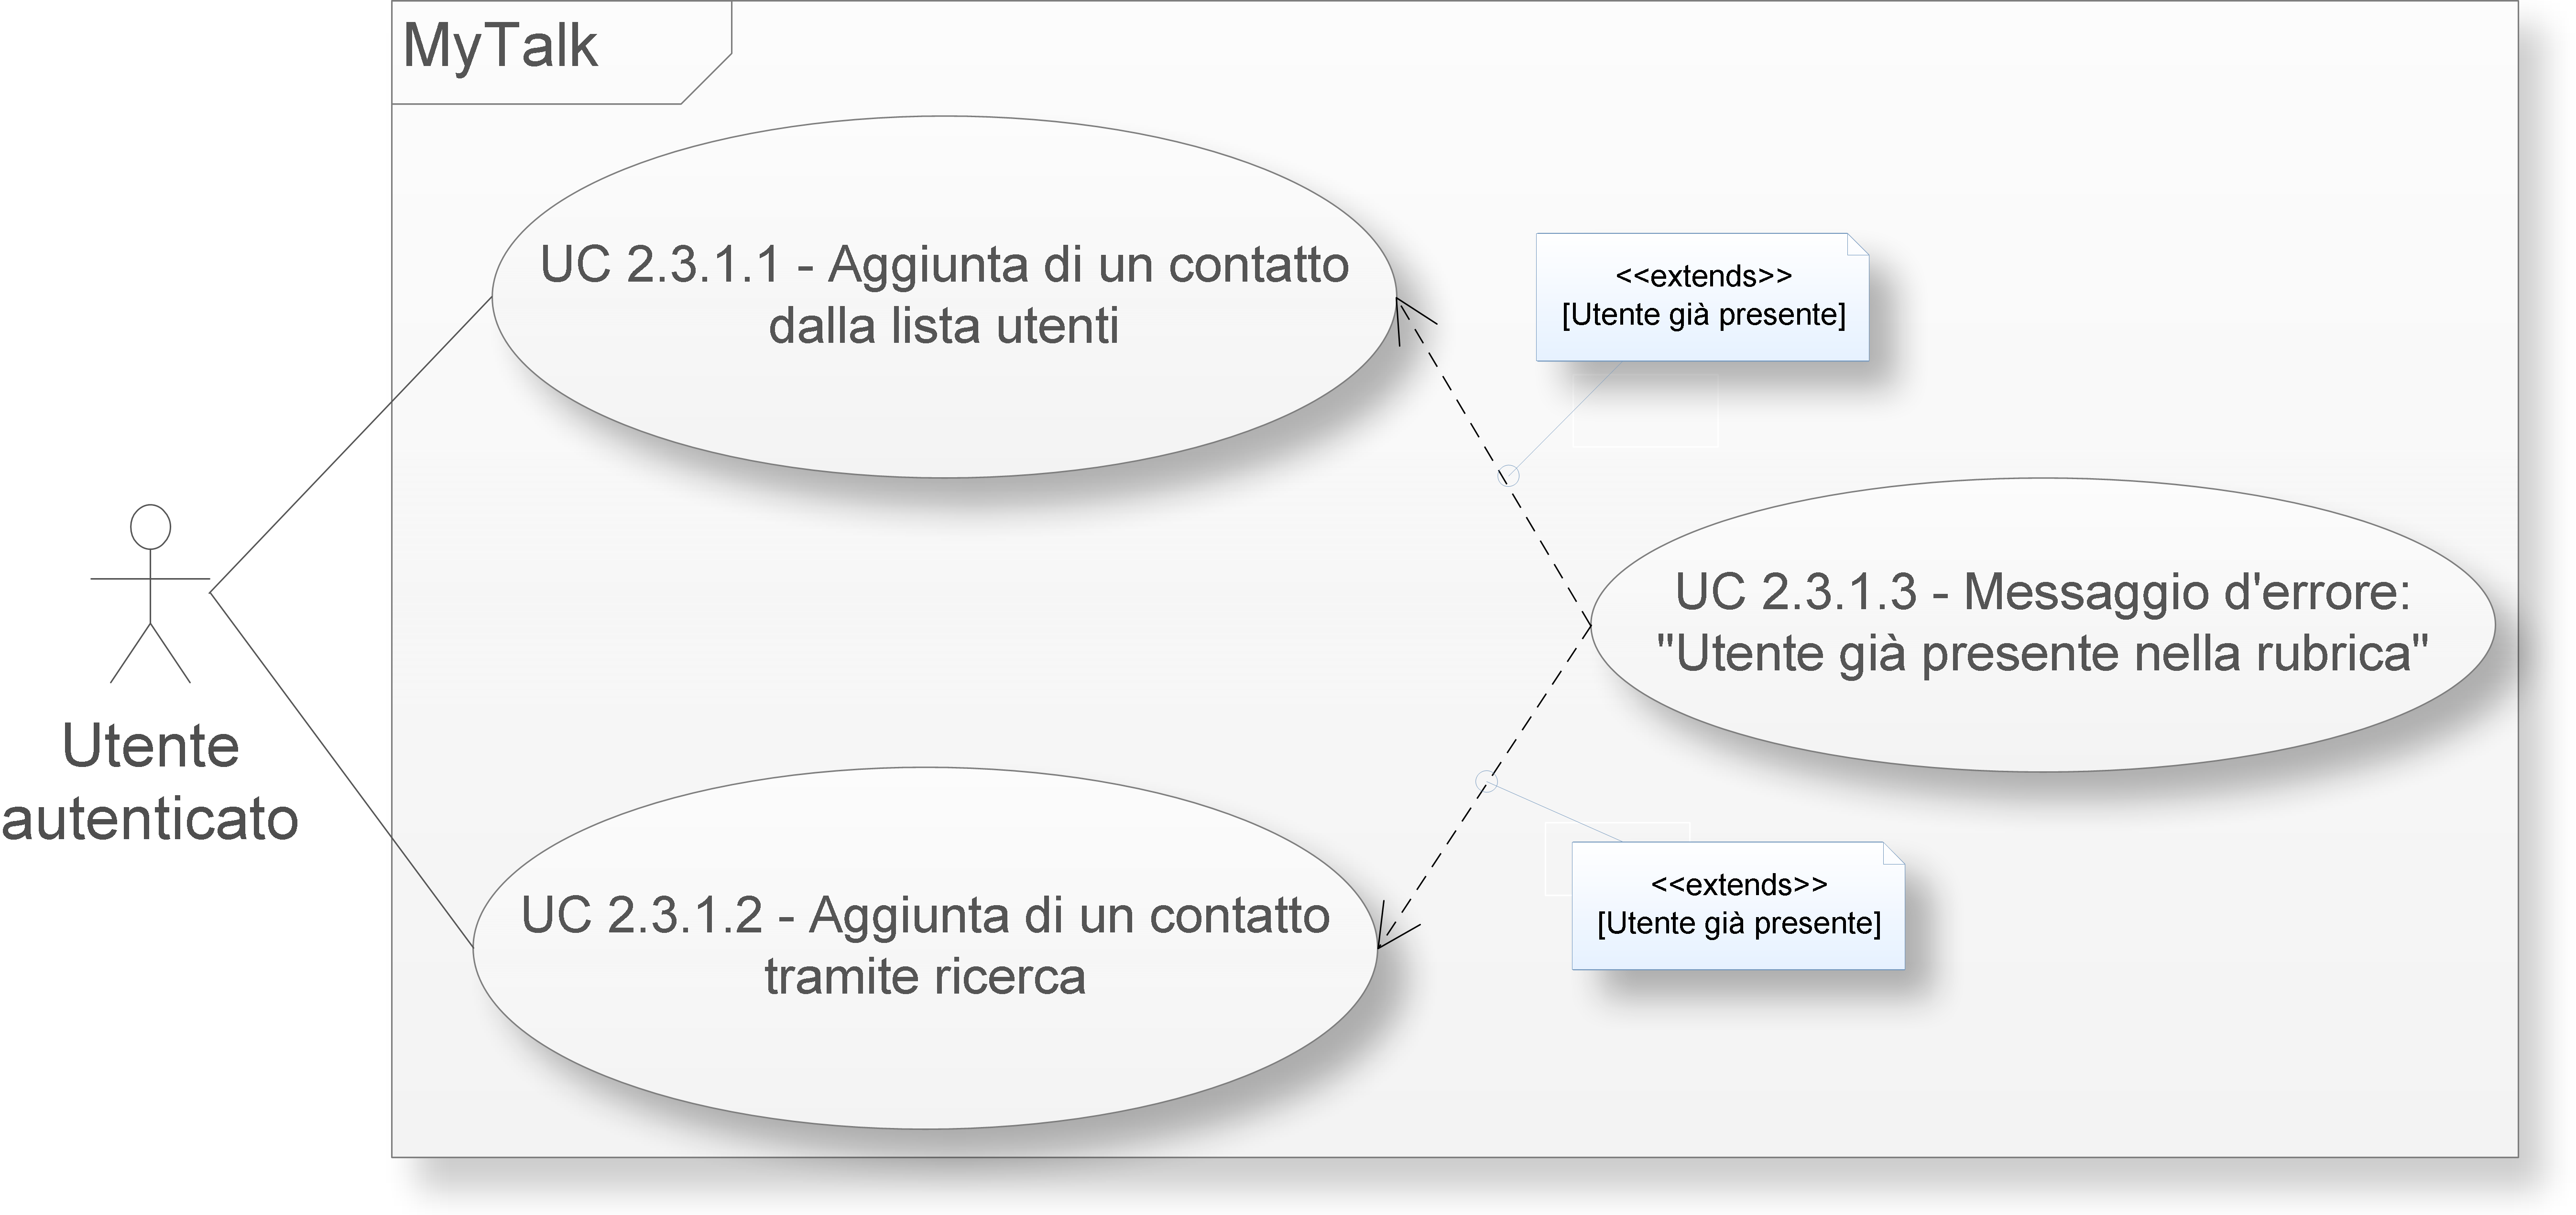
\includegraphics[width=.8\textwidth]{UC2-3-1}
\end{center}
\begin{description}
\item{\scshape\bfseries Attori principali:}Utente autenticato.
\item{\scshape\bfseries Scopo e descrizione:} L'utente aggiunge un contatto alla propria rubrica.
\item{\scshape\bfseries Precondizione:} L'utente e' autenticato al sistema; la lista degli utenti registrati presso il server non è vuota.
\item{\scshape\bfseries Postcondizione:} L'utente ha aggiunto un nuovo contatto nella propria rubrica.
\item{\scshape\bfseries Illustrazione scenario principale:} l'utente può operare l'inserimento seguendo 2 iter. Nel primo caso l'utente seleziona un cotatto direttamente dalla lista degli iscritti; visualizza il profilo del contatto; aggiunge il contatto alla rubrica. Nel secondo caso, l'utente avvia una ricerca del contato basata su un parametro specifico(nome, cognome, mail); seleziona uno dei contatti ritornati dalla ricerca; visualizza il profilo del contatto selezionato infine può aggiunge il contatto alla rubrica.
\item{\scshape\bfseries Illustrazione scenario alternativo:} Se la ricerca del contatto da esito negativo, l'utente puo' operare un'altra ricerca oppure abbandonare l'inserimento del contatto.
\item{\scshape\bfseries Illustrazione scenario alternativo:} Se il contatto selezionato per l'inserimento nella rubrica, è già presente nella rubrica, allora compare un messaggio d'errore che avvisa l'utente dell'inpossibilità di aggiungere il contatto.
\end{description}

\subsection{UC2.4: Gestire segreteria personale}
\begin{center}
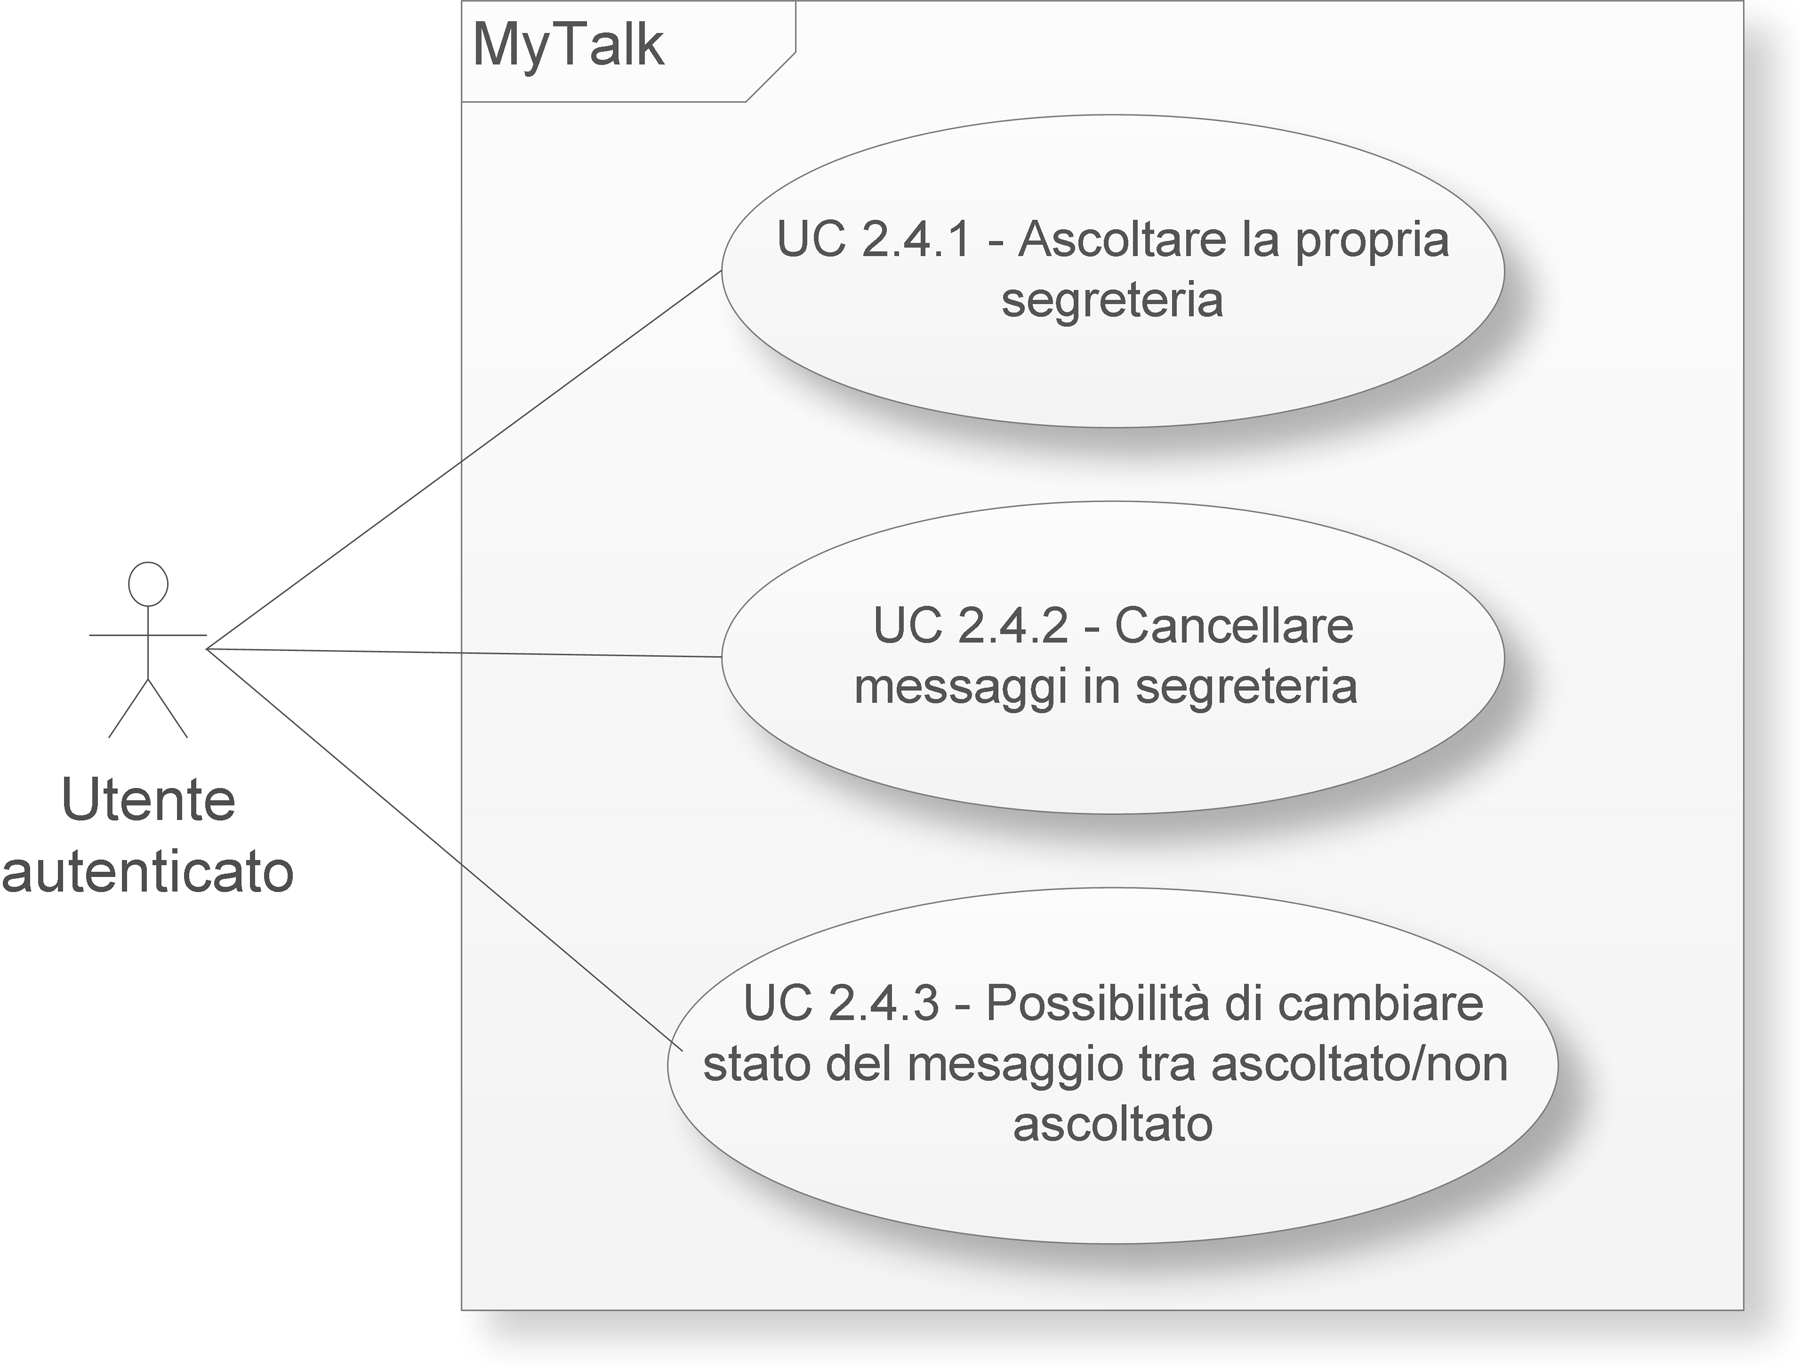
\includegraphics[width=.75\textwidth]{UC2-4}
\end{center}
\begin{description}
\item{\scshape\bfseries Attori principali:}Utente autenticato.
\item{\scshape\bfseries Scopo e descrizione:} L'utente ha a disposizione una segreteria personale che può gestire.
\item{\scshape\bfseries Precondizione:} L'utente ha effettuato la procedura di login ed è quindi autenticato.
\item{\scshape\bfseries Postcondizione:} Il sistema ha eseguito con successo le operazioni richieste dall'utente.
\item{\scshape\bfseries Illustrazione scenario principale:} L'utente si trova nella sezione riguardante la segreteria e può decidere di lasciare un messaggio audio o audio e video nella segreteria di un'altra persona, ascoltare, se presenti, i messaggi lasciati dai propri contatti, e può anche gestirli, cioè eliminarli o contrassegnarli come ascoltati/non ascoltati.
\end{description}

\subsection{UC2.5: Connessione con altri utenti autenticati}
\begin{center}
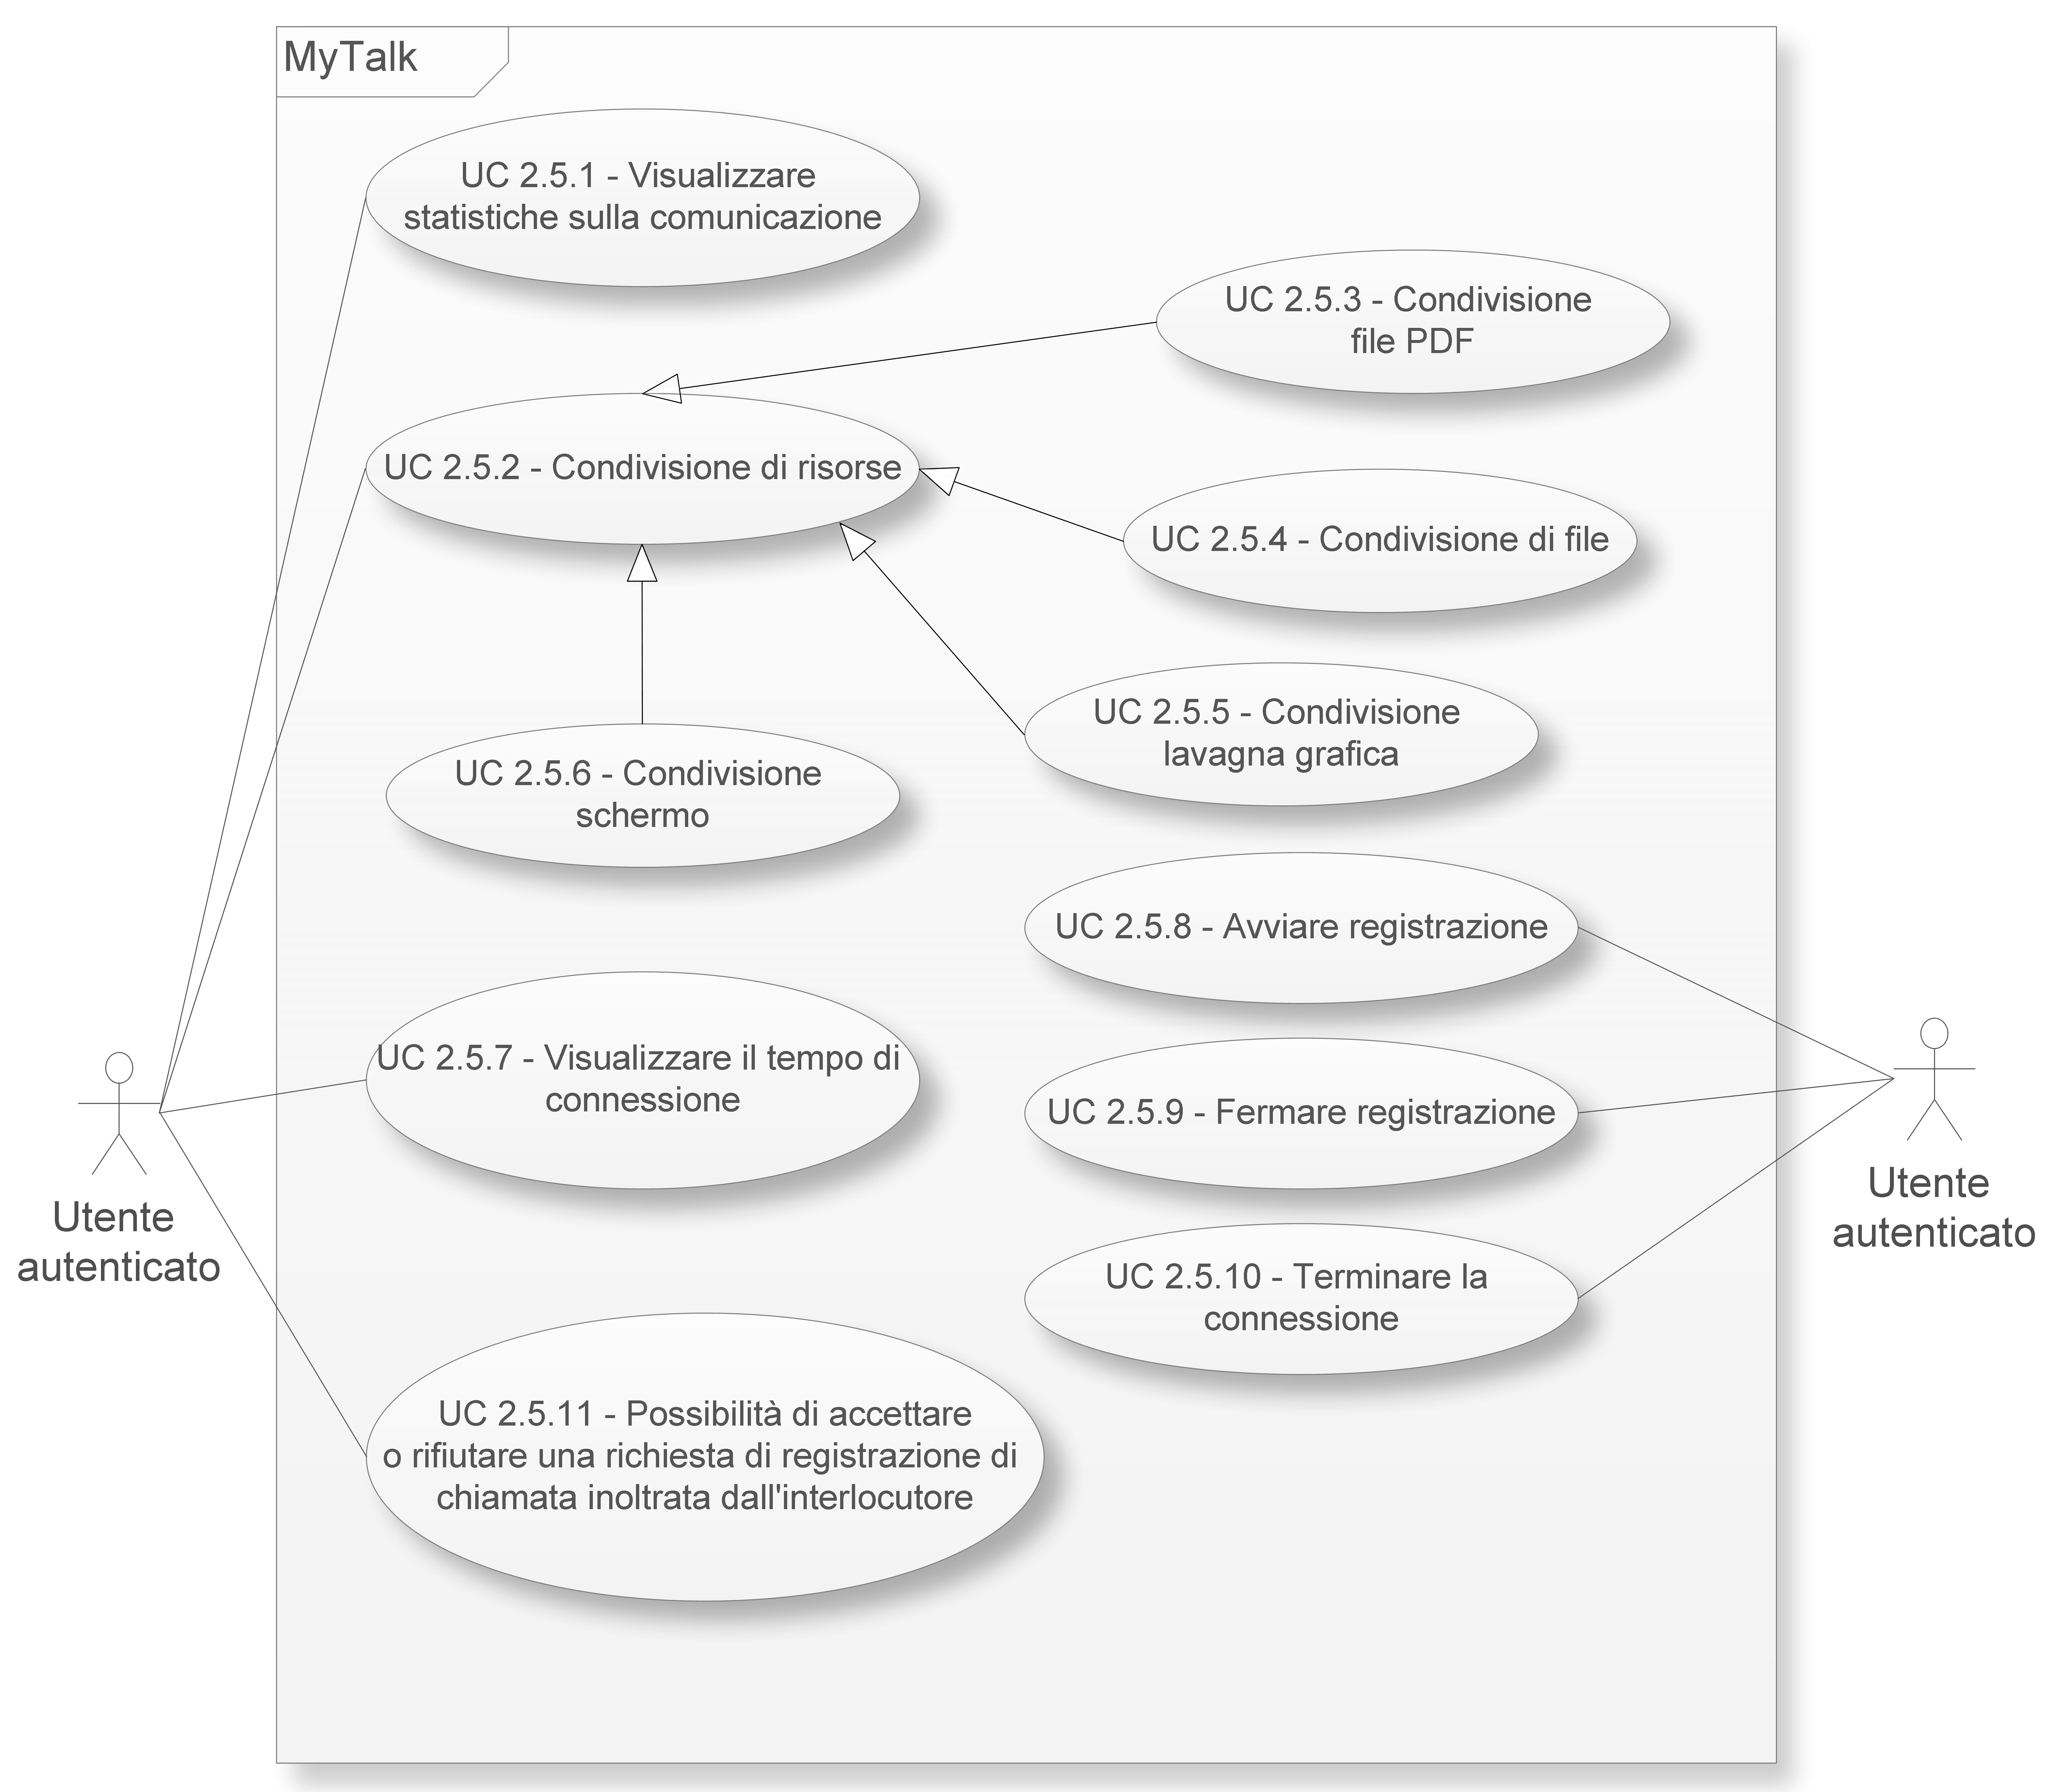
\includegraphics[width=.9\textwidth]{UC2-5}
\end{center}
\begin{description}
\item{\scshape\bfseries Attori principali:}Utente autenticato.
\item{\scshape\bfseries Scopo e descrizione:} Un utente, durante una chiamata audio, audio/video e chat, può eseguire diverse operazioni sulla connessione stabilita.
\item{\scshape\bfseries Precondizione:} L'utente è autenticato nel sistema, ed ha già stabilito una connessione con uno, o più, utenti autenticati.
\item{\scshape\bfseries Postcondizione:} L'utente ha concluso la comunicazione. La causa della terminazione può essere attribuita alla chiusura volontaria della connessione oppure al fatto che l'utente rimane l'unico attivo nella connessione.
\item{\scshape\bfseries Illustrazione scenario principale:} L'utente ha avviato una comunicazione. Mentre questa è in esecuzione, l'utente potrà: visualizzare le statistiche sulla comunicazione; condividere delle risorse dal proprio dispositivo (Condivisione di PDF, invio di file, condivisione di una lavagna grafica, e condivisione dello schermo), visualizzare da quanto tempo è aperta la connessione, avviare e fermare una registrazione, Accettare o rifiutare una richiesta di registrazione inoltrata da un interlocutore. Infine l'utente può decidere di terminare la comunicazione.
\end{description}

\subsection{UC2.5.1: Visualizzazione statistiche sulla comunicazione}
\begin{center}
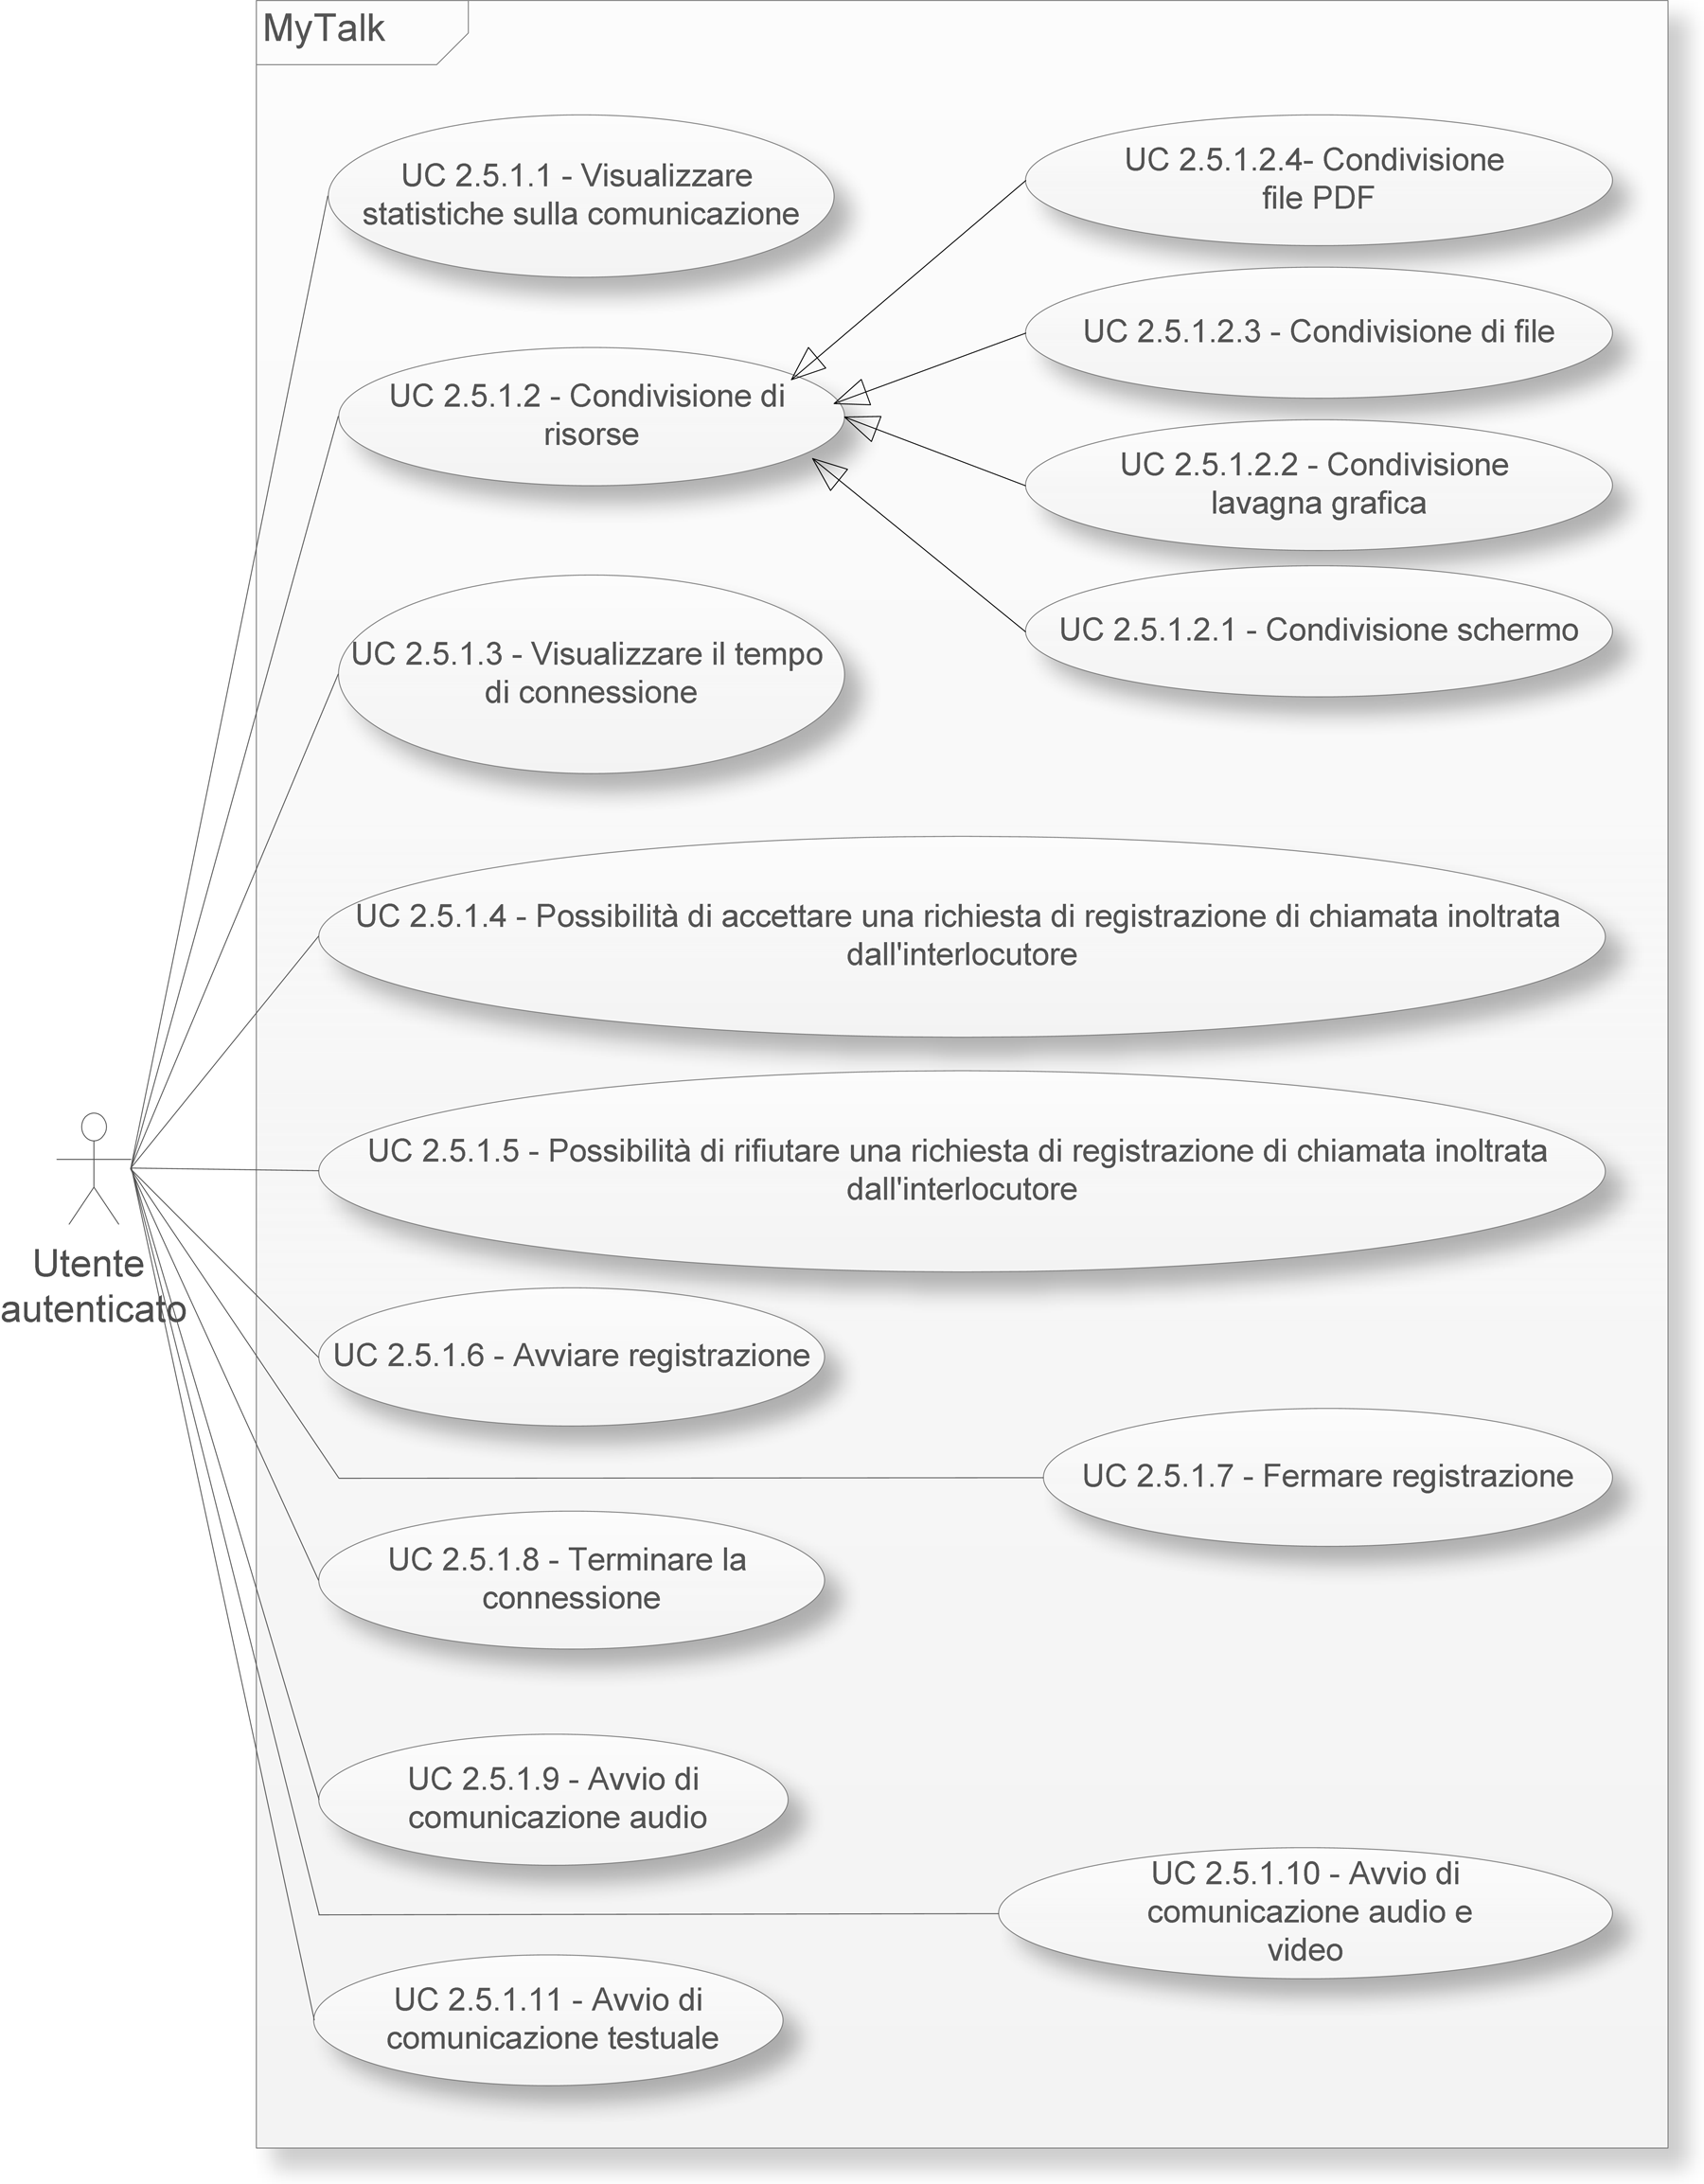
\includegraphics[width=.9\textwidth]{UC2-5-1}
\end{center}
\begin{description}
\item{\scshape\bfseries Attori principali:}Utente autenticato.
\item{\scshape\bfseries Scopo e descrizione:} L'utente visualizza i dettagli della comunicazione con un altro utente.
\item{\scshape\bfseries Precondizione:} L'utente sta comunicando con un altro utente del sistema.
\item{\scshape\bfseries Postcondizione:} L'utente ha visualizzato tutte le informazioni riguardanti la comunicazione.
\item{\scshape\bfseries Illustrazione scenario principale:} L'utente che comincia a comunicare con un altro utente ha a disposizione la visualizzazione di alcune informazioni sulla comunicazione in corso, come la durata della chiamata, il numero di byte ricevuti ed inviati, la latenza ossia il tempo che passa da quando un utente parla a quando l'altro utente sente le parole pronunciate, la velocità di trasmissione dei dati e i frame per secondo (fps) nel caso sia in corso una videochiamata.
\end{description}

\newpage\section{Requisiti}

I requisiti verranno suddivisi in base alla loro priorità. Rispettivamente seguirà la lista dei requisiti obbligatori, facoltativi e desiferabili. Ogni requisito è identificato con il seguente formato RXYZI con:


		\begin{itemize}

			\item \textbf{X}: indica la tipologia dell'utente interessato dal requisito. I possibili valori che X può assumere sono U (utente) oppure S (sistema).

			\item \textbf{Y}: indica la tipologia del requisito, e può assumere i valori: F(funzionale), Q(qualitativo), P(prestazionale), D(dichiarativo).

			\item \textbf{Z}: indica il livello di priorità del requisito. Può assumere i valori O(obbligatorio), \\F(facoltativo), D(desiderabile).

			\item \textbf{I}: indica l'id numerico del requisito, denominato secondo le direttive delle norme di progetto.

		\end{itemize}


		Ogni requisito si può suddividere in sottorequisiti. Tale evento è evidenziato dal valore del campo I, come riportato nelle norme di progetto. Infine i requisiti sono ordinati (nelle proprie sezioni) in base all'ordine crescente del campo numerico I.
\subsection{Requisiti obbligatori}

\rowcolors{1}{lightblue}{llightblue}
\begin{longtable}{lp{.55\textwidth}l}
\hiderowcolors
\toprule Codice & Requisito & Fonte\\
\midrule
\showrowcolors
\endhead
RUFO1.0.0 & L'utente deve potersi autentificare nel server, così da permettere a quest'ultimo di rilevare la sua presenza nel sistema. Il Login dovrà essere gestito con username (indirizzo e-mail) e password. & Interno \\
RUFO2.0.0 & Registrazione del nuovo utente & Capitolato d'appalto \\
RUFO5.0.0 & Possibilità di visualizzare la lista di utenti registrati nel sistema & Capitolato d'appalto \\
RSDO6.0.0 & Gestire le comunicazioni utente tramite WebRTC & Capitolato d'appalto \\
RUFO6.1.0 & Stabilire e gestire una comunicazione audio con un utente in linea & Capitolato d'appalto \\
RUFO6.1.1 & Stabilire una comunicazione audio mediante inserimento d'indirizzo IP & Capitolato d'appalto \\
RUFO6.1.3 & Stabilire una comunicazione audio con un utente registrato e NON presente nella rubrica & Capitolato d'appalto \\
RUFO6.2.0 & Stabilire e gestire  una comunicazione audio/video con un utente & Capitolato d'appalto \\
RUFO6.2.1 & Stabilire una comunicazione audio/video mediante inserimento d'indirizzo IP & Capitolato d'appalto \\
RUFO6.2.3 & Stabilire una comunicazione audio/video con un utente registrato e NON presente nella rubrica & Capitolato d'appalto \\
RUFO7.0.0 & Indicare il tempo di comunicazione & Capitolato d'appalto \\
RUFO8.0.0 & Valutare il numero di byte trasmessi & Capitolato d'appalto \\
RUFO8.1.0 & Valutare il numero di byte inviati & Interno \\
RUFO8.2.0 & Valutare il numero di byte ricevuti & Interno \\
RUFO9.0.0 & Indicare la qualità della linea di trasmissione & Capitolato d'appalto \\
RUFO9.1.0 & Rilevare latenza & Capitolato d'appalto \\
RUFO9.2.0 & Rilevare velocità di trasmissione & Capitolato d'appalto \\
RSDO10.0.0 & L'intero sistema deve essere contenuto in un unica pagina Web & Capitolato d'appalto \\
RSDO10.1.0 & L'interfaccia grafica non deve subire refresh per ogni operazione dell'utente & Interno \\
RSFO11.0.0 & Creare una connessione tra client, mediante l'utilizzo di un server & Capitolato d'appalto \\
RSFO11.1.0 & Utilizzo del protocollo webSocket per creare una connessione tra 2 utenti & Interno \\
RSFO12.0.0 & Gestire gli eventi dell'utente durante la connessione. & Interno \\
RUFO12.3.0 & Chi partecipa alla connessione può togliersi da essa & Interno \\
RSDO22.0.0 & L'applicativo deve funzionare sotto l'ultima versione (23.0.1271.97m) del browser Google Chrome & Capitolato d'appalto \\
\bottomrule
\end{longtable}
\subsection{Requisiti facoltativi}

\rowcolors{1}{lightblue}{llightblue}
\begin{longtable}{lp{.55\textwidth}l}
\hiderowcolors
\toprule Codice & Requisito & Fonte\\
\midrule
\showrowcolors
\endhead
RUFF3.0.0 & Modifica dati utente (ad eccezione dell'indirizzo email) & Interno \\
RUFF4.0.0 & L'utente dovrebbe poter tenere tenere una rubrica personale dove raggruppare i propri contatti. & Interno \\
RUFF4.1.0 & Un utente deve poter inserire utenti dalla propria rubrica. & Capitolato d'appalto \\
RUFF4.2.0 & Eliminare un utente dalla propria rubrica & Interno \\
RUFF4.3.0 & Possibilità di ordinare la rubrica su alcuni parametri rilevanti & Interno \\
RUFF4.4.0 & Possibilità di suddividere la rubrica in gruppi & Interno \\
RUFF4.4.1 & Possibilità di togliere un elemento da un gruppo & Interno \\
RUFF4.4.2 & Possibilità di aggiungere un elemento in un gruppo & Interno \\
RUFF4.4.3 & Possibilità di creare un gruppo & Interno \\
RUFF4.4.4 & Possibilità di eliminare un gruppo & Interno \\
RUFF4.5.0 & Possibilità di esportare in xml la rubrica personale & Interno \\
RUFF4.6.0 & Possibilità di modificare la rubrica importando un file xml & Interno \\
RUFF4.7.0 & Ricerca di un utente nella propria rubrica. & Interno \\
RUFF5.1.0 & Possibilità di cercare un utente dalla lista & Interno \\
RUFF6.1.2 & Stabilire una comunicazione audio con un utente registrato e presente nella rubrica & Capitolato d'appalto \\
RUFF6.1.4 & Promuovere una comunicazione audio avviata con un utente in una comunicazione audio/video & Interno \\
RUFF6.2.2 & Stabilire una comunicazione audio/video con un utente registrato e presente nella rubrica & Capitolato d'appalto \\
RUFF6.2.4 & Declassare una comunicazione audio/video avviata con un utente in una comunicazione solo audio & Interno \\
RUFF6.2.5 & Disattivare la webcam utente pur continuando a ricevere il segnale video proveniente dall'altro capo della comunicazione & Interno \\
RUFF6.3.0 & Disattivare il microfono utente pur continuando a ricevere il segnale video proveniente dall'altro capo della comunicazione & Interno \\
RUFF9.3.0 & Rilevazione frame per secondo & Interno \\
RSFF11.2.0 & Utilizzo del protocollo webSocket per creare una connessione tra più di 2 utenti & Interno \\
RSFF12.1.0 & Estendere la connessione ad altri client & Interno \\
RUFF13.0.0 & Servizio chat testuale & Capitolato d'appalto \\
RUFF13.2.0 & Servizio chat tra più di 2 utenti & Interno \\
RUFF14.0.0 & Registrazione della chiamata & Capitolato d'appalto \\
RUFF14.1.0 & Necessità di autorizzazione dagli utenti della chiamata per poter avviare la registrazione & Interno \\
RUFF14.2.0 & Registrazione audio & Interno \\
RUFF14.3.0 & Possibilità di riascoltare la registrazione & Interno \\
RUFF15.0.0 & L'utente avrà a disposizione una segreteria telefonica. & Interno \\
RUFF15.1.0 & Possibilità di lasciare un audio messaggio in segreteria & Interno \\
RUFF15.2.0 & Possibilità di lasciare un audio/video messaggio in segreteria & Capitolato d'appalto \\
RUFF15.3.0 & Possibilità di ascoltare la propria segreteria & Interno \\
RUFF15.4.0 & Possibilità di cancellare messaggi della segretaria & Interno \\
RUFF15.5.0 & Possibilità di cambiare lo stato del messaggio tra ascoltato/non ascoltato & Interno \\
RUFF16.0.0 & Possibilità di impostare uno stato utente & Interno \\
RUFF17.0.0 & Dare la possibilità di vedere gli stati personali altrui. & Interno \\
RUFF18.0.0 & Creazione di una Blacklist & Interno \\
RUFF19.0.0 & Possibilità di tenere uno storico delle chiamate & Interno \\
RUFF20.0.0 & Condividere risorse & Interno \\
RUFF20.1.0 & Condividere monitor & Interno \\
RUFF20.2.0 & Condivisione pdf & Interno \\
RUFF20.3.0 & Condivisione lavagna grafica. & Interno \\
RUFF20.4.0 & Invio file & Interno \\
RSQF23.0.0 & Verificare che l'applicativo funzioni anche sotto gli altri browser del S.O. Windows & Interno \\
RSQF23.1.0 & Verificare che funzioni con Opera & Capitolato d'appalto \\
RSQF23.2.0 & Verificare che funzioni con Firefox & Capitolato d'appalto \\
RSQF23.3.0 & Verificare che funzioni con Internet Explorer (v9 e superiori) & Capitolato d'appalto \\
RSQF23.4.0 & Verificare che funzioni con Safari & Capitolato d'appalto \\
RSQF24.0.0 & Verificare che l'applicativo funzioni anche sotto gli altri browser del S.O. Linux & Interno \\
RSQF24.1.0 & Verificare che funzioni con Opera & Capitolato d'appalto \\
RSQF24.2.0 & Verificare che funzioni con Firefox & Capitolato d'appalto \\
RSQF24.3.0 & Verificare che funzioni con Chromium & Interno \\
RSQF25.0.0 & Verificare che l'applicativo funzioni anche sotto gli altri browser del S.O. Macintosh & Interno \\
RSQF25.1.0 & Verificare che funzioni con Opera & Capitolato d'appalto \\
RSQF25.2.0 & Verificare che funzioni con Firefox & Capitolato d'appalto \\
RSQF25.3.0 & Verificare che funzioni con Safari & Capitolato d'appalto \\
\bottomrule
\end{longtable}
\subsection{Requisiti desiderabili}

\rowcolors{1}{lightblue}{llightblue}
\begin{longtable}{lp{.55\textwidth}l}
\hiderowcolors
\toprule Codice & Requisito & Fonte\\
\showrowcolors
\midrule
\endhead
RUFD1.1.0 & Gestione password dimenticata & Interno \\
RUFD1.1.1 & Proporre la domanda segreta all'utente & Interno \\
RUFD1.1.2 & Invio di una mail all'utente contenete la password dimenticata & Interno \\
RSDD2.1.0 & L'utente dovrebbe avere una stima della complessità per la propria password. & Capitolato d'appalto \\
RSDD2.2.0 & Convalidare username (e-mail) dell'utente & Interno \\
RSDD2.3.0 & Inserimento dati anagrafici (nome, cognome), immagine e indirizzo email (utilizzato anche come username) & Interno \\
RUFD12.2.0 & Chi crea la connessione può eliminare i membri del gruppo & Interno \\
RUFD13.1.0 & Servizio chat tra 2 utenti & Interno \\
RSQD21.0.0 & Gestione interfaccia grafica in più lingue & Interno \\
\bottomrule
\end{longtable}
\newpage\section{Tracciamento dei requisiti}\label{sec:tracciamento}

\rowcolors{1}{lightblue}{llightblue}
\begin{longtable}{lp{.55\textwidth}l}
\hiderowcolors
\toprule
Codice UC & Nome UC  & Requisito\\
\showrowcolors
\midrule
\endhead
UC1 & Login e registrazione & RUFO1.0.0 \\
 &  & RUFD1.1.0 \\
 &  & RUFD1.1.1 \\
 &  & RUFD1.1.2 \\
 &  & RUFO2.0.0 \\
 &  & RSDD2.1.0 \\
 &  & RSDD2.2.0 \\
 &  & RSDD2.3.0 \\
UC2 & Home screen dell'applicativo & RUFF3.0.0 \\
 &  & RUFF4.0.0 \\
 &  & RUFF4.1.0 \\
 &  & RUFF4.2.0 \\
 &  & RUFF4.3.0 \\
 &  & RUFF4.4.0 \\
 &  & RUFF4.4.1 \\
 &  & RUFF4.4.2 \\
 &  & RUFF4.4.3 \\
 &  & RUFF4.4.4 \\
 &  & RUFF4.5.0 \\
 &  & RUFF4.6.0 \\
 &  & RUFF4.7.0 \\
 &  & RUFO5.0.0 \\
 &  & RUFF5.1.0 \\
 &  & RUFO6.1.0 \\
 &  & RUFO6.1.1 \\
 &  & RUFF6.1.2 \\
 &  & RUFO6.1.3 \\
 &  & RUFF6.1.4 \\
 &  & RUFO6.2.0 \\
 &  & RUFO6.2.1 \\
 &  & RUFF6.2.2 \\
 &  & RUFO6.2.3 \\
 &  & RUFF6.2.4 \\
 &  & RUFF6.2.5 \\
 &  & RUFF6.3.0 \\
 &  & RUFO7.0.0 \\
 &  & RUFO8.0.0 \\
 &  & RUFO8.1.0 \\
 &  & RUFO8.2.0 \\
 &  & RUFO9.0.0 \\
 &  & RUFO9.1.0 \\
 &  & RUFO9.2.0 \\
 &  & RUFF9.3.0 \\
 &  & RSFF12.1.0 \\
 &  & RUFD12.2.0 \\
 &  & RUFO12.3.0 \\
 &  & RUFF13.0.0 \\
 &  & RUFD13.1.0 \\
 &  & RUFF13.2.0 \\
 &  & RUFF14.0.0 \\
 &  & RUFF14.1.0 \\
 &  & RUFF14.2.0 \\
 &  & RUFF15.0.0 \\
 &  & RUFF15.1.0 \\
 &  & RUFF15.2.0 \\
 &  & RUFF15.3.0 \\
 &  & RUFF15.4.0 \\
 &  & RUFF15.5.0 \\
 &  & RUFF16.0.0 \\
 &  & RUFF17.0.0 \\
 &  & RUFF18.0.0 \\
 &  & RUFF19.0.0 \\
 &  & RUFF20.0.0 \\
 &  & RUFF20.1.0 \\
 &  & RUFF20.2.0 \\
 &  & RUFF20.3.0 \\
 &  & RUFF20.4.0 \\
UC1.1 & Login utente & RUFO1.0.0 \\
UC1.2 & Registrazione & RUFO2.0.0 \\
 &  & RSDD2.1.0 \\
 &  & RSDD2.2.0 \\
 &  & RSDD2.3.0 \\
UC1.3 & Recupero della password & RUFD1.1.0 \\
 &  & RUFD1.1.1 \\
 &  & RUFD1.1.2 \\
UC2.1 & Gestione account & RUFF3.0.0 \\
UC2.3 & Gestione della rubrica & RUFF4.0.0 \\
 &  & RUFF4.1.0 \\
 &  & RUFF4.2.0 \\
 &  & RUFF4.3.0 \\
 &  & RUFF4.4.0 \\
 &  & RUFF4.4.1 \\
 &  & RUFF4.4.2 \\
 &  & RUFF4.4.3 \\
 &  & RUFF4.4.4 \\
 &  & RUFF4.5.0 \\
 &  & RUFF4.6.0 \\
 &  & RUFF4.7.0 \\
 &  & RUFO5.0.0 \\
 &  & RUFF5.1.0 \\
 &  & RUFF18.0.0 \\
UC2.4 & Gestire segreteria personale & RUFF15.0.0 \\
 &  & RUFF15.1.0 \\
 &  & RUFF15.2.0 \\
 &  & RUFF15.3.0 \\
 &  & RUFF15.4.0 \\
 &  & RUFF15.5.0 \\
UC2.5 & Connessione con altri utenti autenticati & RUFO6.1.0 \\
 &  & RUFO6.1.1 \\
 &  & RUFF6.1.2 \\
 &  & RUFO6.1.3 \\
 &  & RUFF6.1.4 \\
 &  & RUFO6.2.0 \\
 &  & RUFO6.2.1 \\
 &  & RUFF6.2.2 \\
 &  & RUFO6.2.3 \\
 &  & RUFF6.2.4 \\
 &  & RUFF6.2.5 \\
 &  & RUFF6.3.0 \\
 &  & RUFO7.0.0 \\
 &  & RUFO8.0.0 \\
 &  & RUFO8.1.0 \\
 &  & RUFO8.2.0 \\
 &  & RUFO9.0.0 \\
 &  & RUFO9.1.0 \\
 &  & RUFO9.2.0 \\
 &  & RUFF9.3.0 \\
 &  & RSFO12.0.0 \\
 &  & RSFF12.1.0 \\
 &  & RUFD12.2.0 \\
 &  & RUFO12.3.0 \\
 &  & RUFF13.0.0 \\
 &  & RUFD13.1.0 \\
 &  & RUFF13.2.0 \\
 &  & RUFF14.0.0 \\
 &  & RUFF14.1.0 \\
 &  & RUFF14.2.0 \\
 &  & RUFF20.0.0 \\
 &  & RUFF20.1.0 \\
 &  & RUFF20.2.0 \\
 &  & RUFF20.3.0 \\
 &  & RUFF20.4.0 \\
UC2.3.1 & Aggiungi contatto & RUFF4.1.0 \\
UC2.5.1 & Visualizzazione statistiche sulla comunicazione & RUFO7.0.0 \\
 &  & RUFO8.1.0 \\
 &  & RUFO8.2.0 \\
 &  & RUFO9.0.0 \\
 &  & RUFO9.1.0 \\
 &  & RUFO9.2.0 \\
 &  & RUFF9.3.0 \\
\bottomrule
\end{longtable}
